\documentclass[11pt, fontset=Minion, showoverfull,
bib, mintcode, minted=cache]{marticle}
\UseAbbr{ais}   \UseAbbr{Ais}
\UseAbbr{cpu}   \UseAbbr{Cpu}
\UseAbbr{gmm}   \UseAbbr{Gmm}
\UseAbbr{gpgpu} \UseAbbr{Gpgpu}
\UseAbbr{gpu}   \UseAbbr{Gpu}
\UseAbbr{gui}   \UseAbbr{Gui}
\UseAbbr{io}    \UseAbbr{Io}
\UseAbbr{mcmc}  \UseAbbr{Mcmc}
\UseAbbr{rng}   \UseAbbr{Rng}
\UseAbbr{simd}  \UseAbbr{Simd}
\UseAbbr{sis}   \UseAbbr{Sis}
\UseAbbr{smc}   \UseAbbr{Smc}
\UseAbbr{smp}   \UseAbbr{Smp}
\UseAbbr{ess}   \UseAbbr{Ess}

\UseAbbr[\aocl][\sffamily\scshape]{amd app OpenCL}
\UseAbbr[\biips][\sffamily]{BiiPS}
\UseAbbr[\blitz][\sffamily]{Blitz++}
\UseAbbr[\boost][\sffamily]{Boost}
\UseAbbr[\bugs][\sffamily\scshape]{bugs}
\UseAbbr[\cilk][\sffamily]{Cilk Plus}
\UseAbbr[\cmake][\sffamily]{CMake}
\UseAbbr[\clang][\sffamily]{clang}
\UseAbbr[\cppne][\sffamily]{C++98}
\UseAbbr[\cppoo][\sffamily]{C++11}
\UseAbbr[\cpp][\sffamily]{C++}
\UseAbbr[\doxygen][\sffamily]{Doxygen}
\UseAbbr[\gcc][\sffamily\scshape]{gcc}
\UseAbbr[\git][\sffamily]{Git}
\UseAbbr[\html][\sffamily\scshape]{html}
\UseAbbr[\icpc][\sffamily]{Intel C++ Compiler}
\UseAbbr[\iocl][\sffamily]{Intel OpenCL}
\UseAbbr[\libbi][\sffamily]{LibBi}
\UseAbbr[\libcpp][\sffamily]{libc++}
\UseAbbr[\mpi][\sffamily\scshape]{mpi}
\UseAbbr[\msvc][\sffamily]{Microsoft Visual C++}
\UseAbbr[\opencl][\sffamily]{OpenCL}
\UseAbbr[\openmp][\sffamily]{OpenMP}
\UseAbbr[\random][\sffamily]{Random123}
\UseAbbr[\rlang][\sffamily]{R}
\UseAbbr[\smctc][\sffamily\scshape]{smctc}
\UseAbbr[\tbb][\sffamily]{Intel Threading Building Blocks}
\UseAbbr[\vsmc][\sffamily]{vSMC}

\def\LinkAbbr#1#2{
  \csgdef{l#1}{\href{#2}{\csuse{#1}\xspace}}
  \csgdef{f#1}{\href{#2}{\csuse{#1}}\footnote{\url{#2}}\xspace}%
}
\LinkAbbr{aocl}{http://developer.amd.com/tools-and-sdks/opencl-zone/}
\LinkAbbr{biips}{https://alea.bordeaux.inria.fr/biips/doku.php}
\LinkAbbr{blitz}{http://blitz.sourceforge.net}
\LinkAbbr{boost}{http://www.boost.org}
\LinkAbbr{bugs}{http://www.mrc-bsu.cam.ac.uk/software/bugs/}
\LinkAbbr{cilk}{https://www.cilkplus.org}
\LinkAbbr{clang}{http://clang.llvm.org}
\LinkAbbr{cmake}{http://www.cmake.org}
\LinkAbbr{doxygen}{http://www.stack.nl/~dimitri/doxygen/}
\LinkAbbr{gcc}{https://gcc.gnu.org}
\LinkAbbr{git}{http://git-scm.com}
\LinkAbbr{icpc}{https://software.intel.com/en-us/c-compilers}
\LinkAbbr{iocl}{https://software.intel.com/en-us/intel-opencl}
\LinkAbbr{libbi}{http://libbi.org}
\LinkAbbr{libcpp}{http://libcxx.llvm.org}
\LinkAbbr{mpi}{http://www.mpi-forum.org}
\LinkAbbr{msvc}{https://msdn.microsoft.com/en-us/vstudio/hh386302.aspx}
\LinkAbbr{opencl}{https://www.khronos.org/opencl/}
\LinkAbbr{openmp}{http://openmp.org/wp/}
\LinkAbbr{random}{http://www.deshawresearch.com/resources_random123.html}
\LinkAbbr{rlang}{http://www.r-project.org}
\LinkAbbr{smctc}{http://www2.warwick.ac.uk/fac/sci/statistics/staff/academic-research/johansen/smctc/}
\LinkAbbr{tbb}{https://www.threadingbuildingblocks.org}

\UseMathCal{D}
\UseMathCal{G}
\UseMathCal{M}
\UseMathCal{N}
\UseMathBold{y}
\def\rnd#1#2{\ensuremath{\frac{\diff#1}{\diff#2}}\xspace}
\def\xpos{x_{\mathrm{pos}}}
\def\ypos{y_{\mathrm{pos}}}
\def\xvel{x_{\mathrm{vel}}}
\def\yvel{y_{\mathrm{vel}}}
\def\xobs{x_{\mathrm{obs}}}
\def\yobs{y_{\mathrm{obs}}}

\def\STATESKIP{\hskip2em}

% minted
\usemintedstyle{solarizedlight}
\newminted{cpp}{}
\newmintinline{cpp}{}
\newminted{sh}{}
\newmintinline{sh}{}

% biblatex
\renewbibmacro{in:}
{\ifentrytype{article}{}{\printtext{\bibstring{in}\intitlepunct}}}
\addbibresource{tutorial.bib}


\title{\protect\vsmc{} -- Parallel Sequential Monte Carlo in C++}
\author{Yan Zhou}

\begin{document}

\maketitle

\section{Introduction}
\label{sec:Introduction}

\emph{Sequential Monte Carlo} (\smc) is a class of sampling algorithms that
combine importance sampling and resampling. They have been used as ``particle
filters'' to solve optimal filtering problems; see, for example,
\textcite{Cappe:2007hz} and \textcite{Doucet:2011us} for recent reviews. They
are also used in a static setting where a target distribution is of interest,
for example, a posterior distribution in Bayesian modeling. This was proposed
by \textcite{DelMoral:2006hc} and developed by \textcite{Peters:2005wh} and
\textcite{DelMoral:2006wv}. This framework involves the construction of a
sequence of artificial distributions on spaces of increasing dimensions which
admit the distributions of interest as particular marginals.

\Smc algorithms are perceived as being difficult to implement while general
tools were not available until the development of \fsmctc \parencite{smctc}.
\Smc algorithms admit natural and scalable parallelization. However, there are
only parallel implementations of \smc algorithms for many problem specific
applications. \textcite{Lee:2010fm} studied the parallelization of \smc
algorithms on \gpu{}s with some generality. There are few tools to implement
generic \smc algorithms on parallel hardware though multicore \cpu{}s are very
common today and computing on specialized hardware such as \gpu{}s are
attracting considerable interests.

The purpose of the current work is to provide a framework for implementing
generic \smc algorithms on both sequential and parallel hardware. There are
two main goals of the presented framework. The first is reusability. It will
be demonstrated that the same implementation source can be used to build a
serialized sampler, or using different programming models (for example,
\fopenmp and \ftbb) to build parallelized samplers for multicore \cpu{}s. They
can be scaled for clusters using \fmpi with few modifications. And with a
little effort they can also be used to build parallelized samplers on
specialized massive parallel hardware such as \gpu{}s using \fopencl. The
second is extensibility. It is possible to write a backend for \vsmc to use
new parallel programming models while reusing existing implementations. It is
also possible to enhance the library to improve performance for specific
applications. Almost all components of the library can be reimplemented by
users and thus if the default implementation is not suitable for a specific
application, they can be replaced while being integrated with other components
seamlessly.

Though \vsmc is a new library designed from the ground up, it has some
similarity to the aforementioned \lsmctc library, which is by intention. For
example, they both use user defined callbacks to perform application specific
operations while the library only implements tasks that are common to all
samplers. However, there are also significant differences. First of all, \vsmc
allows easy implementation of parallelized algorithms. The library is also
more flexible and enjoys better performance. The reusability and extensibility
of \vsmc lead to better algorithm implementation design, such that less
duplicate work needs to be done for different algorithms. Both flexibility and
better performance are made possible through the use of template
metaprogramming, a technique pioneered by \fblitz. Some differences of the two
libraries and the advantage of the approach of \vsmc will be discussed when
features are introduced in section~\ref{sec:The vSMC library}. A more detailed
comparison can be found in appendix~\appref{sec:vsmc and smctc}. We will not
elaborate this topic further before the \smc algorithms and the library are
properly introduced in the following sections.

\section{Sequential Monte Carlo}
\label{sec:Sequential Monte Carlo}

\subsection{Sequential importance sampling and resampling}
\label{sub:Sequential importance sampling and resampling}

\emph{Importance sampling} is a technique which allows the calculation of the
expectation of a function $\varphi$ with respect to a distribution $\pi$ using
samples from some other distribution $\eta$ with respect to which $\pi$ is
absolutely continuous, based on the identity,
\begin{equation}
  \Exp_{\pi}[\varphi(X)]
  = \int\varphi(x)\pi(x)\intd x
  = \int\frac{\varphi(x)\pi(x)}{\eta(x)}\eta(x)\intd x
  = \Exp_{\eta}\Square[Big]{\frac{\varphi(X)\pi(X)}{\eta(X)}}.
\end{equation}
Let $\{X^{(i)}\}_{i=1}^N$ be samples from $\eta$, then
$\Exp_{\pi}[\varphi(X)]$ can be approximated by,
\begin{equation}
  \hat\varphi_1 =
  \frac{1}{N}\sum_{i=1}^N\frac{\varphi(X^{(i)})\pi(X^{(i)})}{\eta(X^{(i)})}.
\end{equation}
In practice, $\pi$ and $\eta$ are often only known up to some normalizing
constants, which can be estimated using the same samples. Let $w^{(i)} =
\pi(X^{(i)})/\eta(X^{(i)})$, then we have
\begin{equation}
  \hat\varphi_2 =
  \frac{\sum_{i=1}^Nw^{(i)}\varphi(X^{(i)})}{\sum_{i=1}^Nw^{(i)}},
\end{equation}
or
\begin{equation}
  \hat\varphi_3 = \sum_{i=1}^NW^{(i)}\varphi(X^{(i)})
\end{equation}
where $W^{(i)}\propto w^{(i)}$ and are normalized such that $\sum_{i=1}^N
W^{(i)} = 1$.

\emph{Sequential importance sampling} (\sis) generalizes the importance
sampling technique for a sequence of distributions $\{\pi_t\}_{t\ge0}$ defined
on spaces $\{\prod_{k=0}^tE_k\}_{t\ge0}$. At time $t = 0$, the samples
$\{X_0^{(i)}\}_{i=1}^N$ are generated from $\eta_0$ and the weights are
calculated as $W_0^{(i)} \propto \pi_0(X_0^{(i)})/\eta_0(X_0^{(i)})$. At time
$t\ge1$, each sample $X_{0:t-1}^{(i)}$, usually termed \emph{particles} in the
literature, is extended to $X_{0:t}^{(i)}$ by a proposal distribution
$q_t(\cdot|X_{0:t-1}^{(i)})$. And the weights are recalculated as $W_t^{(i)}
\propto \pi_t(X_{0:t}^{(i)})/\eta_t(X_{0:t}^{(i)})$ where
\begin{equation}
  \eta_t(X_{0:t}^{(i)}) =
  \eta_{t-1}(X_{0:t-1}^{(i)})q_t(X_{0:t}^{(i)}|X_{0:t-1}^{(i)}),
\end{equation}
and
\begin{align}
  W_t^{(i)} \propto \frac{\pi_t(X_{0:t}^{(i)})}{\eta_t(X_{0:t}^{(i)})}
  &= \frac{\pi_t(X_{0:t}^{(i)})\pi_{t-1}(X_{0:t-1}^{(i)})}
  {\eta_{t-1}(X_{0:t-1}^{(i)})q_t(X_{0:t}^{(i)}|X_{0:t-1}^{(i)})
    \pi_{t-1}(X_{0:t-1}^{(i)})} \notag\\
  &= \frac{\pi_t(X_{0:t}^{(i)})}
  {q_t(X_{0:t}^{(i)}|X_{0:t-1}^{(i)})\pi_{t-1}(X_{0:t-1}^{(i)})}W_{t-1}^{(i)}.
  \label{eq:si}
\end{align}
The importance sampling estimate of $\Exp_{\pi_t}[\varphi_t(X_{0:t})]$ can be
obtained using $\{W_t^{(i)},X_{0:t}^{(i)}\}_{i=1}^N$.

However this approach fails as $t$ becomes large. The weights tend to become
concentrated on a few particles as the discrepancy between $\eta_t$ and
$\pi_t$ becomes larger. \emph{Resampling} techniques are applied such that, a
new particle system $\{\bar{W}_t^{(i)},\bar{X}_{0:t}^{(i)}\}_{i=1}^M$ with the
following property is generated,
\begin{equation}
  \Exp\Square[Big]{\sum_{i=1}^M\bar{W}_t^{(i)}\varphi_t(\bar{X}_{0:t}^{(i)})}
  = \Exp\Square[Big]{\sum_{i=1}^NW_t^{(i)}\varphi_t(X_{0:t}^{(i)})}.
  \label{eq:resample}
\end{equation}
In practice, the resampling algorithm is usually chosen such that $M = N$ and
$\bar{W}^{(i)} = 1/N$ for $i=1,\dots,N$. Resampling can be performed at each
time $t$ or adaptively based on some criteria of the discrepancy. One popular
quantity used to monitor the discrepancy is the \emph{effective sample size}
(\ess), introduced by \textcite{Liu:1998iu}, defined as
\begin{equation}
  \ess_t = \frac{1}{\sum_{i=1}^N (W_t^{(i)})^2},
\end{equation}
where $\{W_t^{(i)}\}_{i=1}^N$ are normalized weights. The value of $\ess_t$
tells us the accumulated mismatch between the sample distribution and the
target distribution. Intuitively, when the sample distribution is close to the
target distribution, most weights will be close to $1/N$ and $\ess_t$ will be
close to $N$. In the special case of the samples being generated directly from
the target distribution, the weights are all exactly $1/N$ and $\ess_t$ is
exactly $N$. On the other hand, an extreme small value of $\ess_t$ suggests
that most weights are close to zero while a few are close to one. In this
situation, those few particles can have overwhelming effects on the sampler.
Therefore it is desired to control the sampler such that $\ess_t$ does not
fall below certain threshold by performing resampling regularly. However,
since resampling can be a computational intensive operation, and a bottleneck
to parallel performance, it is also desired to avoid resampling unless it is
necessary. It is a common practice to perform resampling only when $\ess_t\le
\alpha N$ where $\alpha\in[0,1]$. There are little theoretical guidelines on
the choosing of the threshold $\alpha$. However, $\alpha = 0.5$ is often seen
in practice, for example, see \textcite{Jasra:2010eh}.

A common practice of resampling is to replicate particles with large weights
and discard those with small weights. In other words, instead of generating
random samples $\{\bar{X}_{0:t}^{(i)}\}_{i=1}^N$ directly, random samples of
integers $\{R^{(i)}\}_{i=1}^N$ are generated, such that $R^{(i)} \ge 0$ for $i
= 1,\dots,N$ and $\sum_{i=1}^N R^{(i)} = N$. And each particle $X_{0:t}^{(i)}$
is replicated $R^{(i)}$ times in the new particle system. The distribution of
$\{R^{(i)}\}_{i=1}^N$ shall fulfill the requirement of
Equation~\ref{eq:resample}. One such distribution is a multinomial
distribution of size $N$ and weights $(W_t^{(i)},\dots,W_t^{(N)})$. See
\textcite{Douc:2005wa} for some commonly used resampling algorithms.

\subsection[SMC samplers]{\protect\smc samplers}
\label{sub:SMC Samplers}

\Smc samplers allow us to obtain, iteratively, collections of weighted samples
from a sequence of distributions $\{\pi_t\}_{t\ge0}$ over essentially any
random variables on some spaces $\{E_t\}_{t\ge0}$, by constructing a sequence
of auxiliary distributions $\{\tilde\pi_t\}_{t\ge0}$ on spaces of increasing
dimensions, $\tilde\pi_t(x_{0:t})=\pi_t (x_t) \prod_{s=0}^{t-1}
L_s(x_{s+1},x_s)$, where the sequence of Markov kernels $\{L_s\}_{s=0}^{t-1}$,
termed the \emph{backward kernels}, is formally arbitrary but critically
influences the estimator variance. See \textcite{DelMoral:2006hc} for further
details and guidance on the selection of these kernels.

Standard sequential importance sampling and resampling algorithms can then be
applied to the sequence of synthetic distributions, $\{\tilde\pi_t\}_{t\ge0}$.
At time $t - 1$, assume that a set of weighted particles
$\{W_{t-1}^{(i)},X_{0:t-1}^{(i)}\}_{i=1}^N$ approximating $\tilde\pi_{t-1}$ is
available, then at time $t$, the path of each particle is extended with a
Markov kernel say, $K_t(x_{t-1}, x_t)$ and the set of particles
$\{X_{0:t}^{(i)}\}_{i=1}^N$ reach the distribution $\eta_t(X_{0:t}^{(i)}) =
\eta_0(X_0^{(i)})\prod_{k=1}^tK_t(X_{t-1}^{(i)}, X_t^{(i)})$, where $\eta_0$
is the initial distribution of particles. To correct the discrepancy between
$\eta_t$ and $\tilde\pi_t$, Equation~\ref{eq:si} is applied and in this case,
\begin{equation}
  W_t^{(i)} \propto \frac{\tilde\pi_t(X_{0:t}^{(i)})}{\eta_t(X_{0:t}^{(i)})}
  = \frac{\pi_t(X_t^{(i)})\prod_{s=0}^{t-1}L_s(X_{s+1}^{(i)}, X_s^{(i)})}
  {\eta_0(X_0^{(i)})\prod_{k=1}^tK_k(X_{k-1}^{(i)},X_k^{(i)})}
  \propto \tilde{w}_t(X_{t-1}^{(i)}, X_t^{(i)})W_{t-1}^{(i)},
\end{equation}
where $\tilde{w}_t$, termed the \emph{incremental weights}, are calculated as,
\begin{equation}
  \tilde{w}_t(X_{t-1}^{(i)},X_t^{(i)}) =
  \frac{\pi_t(X_t^{(i)})L_{t-1}(X_t^{(i)}, X_{t-1}^{(i)})}
  {\pi_{t-1}(X_{t-1}^{(i)})K_t(X_{t-1}^{(i)}, X_t^{(i)})}.
\end{equation}
If $\pi_t$ is only known up to a normalizing constant, say $\pi_t(x_t) =
\gamma_t(x_t)/Z_t$, then we can use the \emph{unnormalized} incremental
weights,
\begin{equation}
  w_t(X_{t-1}^{(i)},X_t^{(i)}) =
  \frac{\gamma_t(X_t^{(i)})L_{t-1}(X_t^{(i)}, X_{t-1}^{(i)})}
  {\gamma_{t-1}(X_{t-1}^{(i)})K_t(X_{t-1}^{(i)}, X_t^{(i)})},
\end{equation}
for importance sampling. Further, with the \emph{normalized} weights from the
last iterations, $\{W_{t-1}^{(i)}\}_{i=1}^N$, we can estimate the ratio of
normalizing constant $Z_t/Z_{t-1}$ by,
\begin{equation}
  \frac{\hat{Z}_t}{Z_{t-1}} =
  \sum_{i=1}^N W_{t-1}^{(i)}w_t(X_{t-1}^{(i)},X_t^{(i)}).
\end{equation}
Sequentially, the normalizing constant between initial distribution $\pi_0$
and some target $\pi_T$, $T\ge1$ can be estimated. See
\textcite{DelMoral:2006hc} for details on  calculating the incremental
weights. In particular, when $K_t$ is invariant to $\pi_t$, and an
approximated suboptimal backward kernel
\begin{equation}
  L_{t-1}(x_t, x_{t-1}) = \frac{\pi(x_{t-1})K_t(x_{t-1}, x_t)}{\pi_t(x_t)},
\end{equation}
is used, the unnormalized incremental weights are
\begin{equation}
  w_t(X_{t-1}^{(i)},X_t^{(i)}) =
  \frac{\gamma_t(X_{t-1}^{(i)})}{\gamma_{t-1}(X_{t-1}^{(i)})}.
  \label{eq:inc_weight_mcmc}
\end{equation}

\subsection[SMC parallel]{Parallel implementations of \protect\smc algorithms}
\label{sub:SMC parallel}

Parallel computing is a form of computation in which many calculations are
carried out simultaneously. It operates on the principle that large problems
can be divided into \emph{independent} smaller ones and can be solved
\emph{concurrently} (``in parallel''). There are many benefits of parallel
computing, ranging from power efficiency to improved usage of memory. However,
the most relevant one here is perhaps that one can perform the same amount of
computational work with less time. In the ideal (and much simplified)
situation, assuming that there are $K$ identical computing units that can
perform computational tasks independently at the same time, and the total
amount of work can be evenly divided into $K$ independent smaller problems,
then it is possible to finish the same amount of work with time $T/K$, where
$T$ is the time required to complete the work sequentially using only one of
the computing units. The key point here is that those computational tasks are
\emph{independent} of each other. If one task requires the finishing of
another, than those two tasks has to be performed in a particular order, and
essentially cannot be performed concurrently.

In the particular context of \smc algorithms. The updating of the particles
according to a transition kernel can be carried out independently. That is, it
is not important that the particles have to be updated in a particular order.
Therefore, in the above ideal scenario, each computing unit can perform the
computation of updating $N/K$ particles, where $N$ is the total number of
particles. Other steps of the algorithm, such as calculation of the weights
can also be performed in parallel. It is often the case, though unfortunately
not always, that these tasks consumes the most of the computational time of a
given \smc algorithm. By parallelizing these tasks, the algorithm may require
considerably less time to complete. The independence of operations that update
each particle makes parallel computing of particular interest in the context
of \smc related researches.

However, implementing parallelized algorithms is more difficult than
sequential ones for at least two important reasons. First, users often have to
learn new programming models. They can be compiler or language specific
constructs or new libraries. Second, and more importantly, as mentioned
before, dependencies between computations prevent parallelization. And if
ignored, such issues result in incorrect implementations of algorithms.
Without going into technical details, sequential implementations often
implicitly comply with these dependency requirements, while parallel
implementations usually do not. When two tasks are assigned to two computing
units to be carried out concurrently, there is no guarantee that they will be
performed in any particular order without proper programming constructs. Some
of such dependencies are easy to see. For example, in some \smc algorithms,
the calculation of weights need to be performed after the particles being
updated. And users are less likely to attempt to perform these two tasks in
parallel. Others might be less obvious. For example, consider reading weight
$W_t^{(i)}$ and updating weight $W_t^{(j)}$ with $i \ne j$. It might first
appears that these two tasks are independent. However, when the value of
$W_t^{(i)}$ is needed, the value of $\sum_{i=1}^N W_t^{(i)}$ is often also
needed or otherwise $W_t^{(i)}$ need to be the \emph{normalized} weight. And
changing the value of $W_t^{(j)}$ changes the value of $\sum_{i=1}^N
W_t^{(i)}$ or the normalized weights. Therefore, in general there need to be a
well defined order of these two tasks.

The \vsmc library attempts to help users implement parallelized \smc
algorithms while avoiding these two difficulties. First, it abstracts many
parallel programming models such that users do not have to know the technical
details of parallel constructs. Good understanding of \cpp programming is
sufficient for using the library. Second, it also imposes certain
restrictions, such that users are less likely to encounter some dependency
issues. For example, through the interface of the library, it is impossible to
update a single weight $W_t^{(j)}$ while reading another. Of course, as usual
with programming, there are ways to work around such restrictions. And the
library does provide facilities such that more advanced users can easily
implement algorithms when these restrictions are getting in the way.

It should be also noted that not all tasks of a given \smc algorithm can be
parallelized, at least not easily, for example, some resampling algorithms.
Moreover, some operations, such as computing the \ess or the normalized
weights $\{W_t^{(i)}\}_{i=1}^N$, which involves simple summations, can be
parallelized, but not necessarily efficient. In reality, assigning tasks to
different computing units has its own computational cost. And when such cost
is non-trivial when compared to the tasks themselves, a parallelized
implementation can cost more time than a sequential one. The \vsmc library
does not attempt to parallelize these operations. Instead, it provides default
sequential implementations and interfaces for users to provide specialized
implementations when they are desired. Limited by the scope, in this paper
only the most common usage scenarios of the library are introduced.

\subsection{Other sequential Monte Carlo algorithms}
\label{sub:Other sequential Monte Carlo algorithms}

Some other commonly used sequential Monte Carlo algorithms can be viewed as
special cases of algorithms introduced above. The annealed importance sampling
(\ais; \textcite{Neal:2001we}) can be viewed as \smc samplers without
resampling.

Particle filters as seen in the physics and signal processing literature, can
also be interpreted as the sequential importance sampling and resampling
algorithms. See \textcite{Doucet:2011us} for a review of this topic. A simple
particle filter example is used in section~\ref{sub:A simple particle filter}
to demonstrate basic features of the \vsmc library.

\section[Using the vSMC library]{Using the \protect\vsmc library}
\label{sec:Using the vSMC library}

\subsection{Overview}

The \vsmc library uses templates of \cpp to implement generic \smc algorithms.
This library is formed by a few major modules listed below. Some features not
included in these modules are introduced later in context.
\begin{description}
  \item[Core] The highest level of abstraction of \smc samplers. Users
    interact with classes defined within this module to create and manipulate
    \smc samplers. Classes in this module include \cppinline{Sampler},
    \cppinline{Particle} and others. These classes use user defined callback
    functions or callable objects, such as functors, to perform problem
    specific operations, such as updating particle values and weights. This
    module is documented in section~\ref{sub:Core module}.
  \item[Symmetric Multiprocessing (\smp)] This is the form of computing most
    people use everyday, including multiprocessor workstations, multicore
    desktops and laptops. Classes within this module make it possible to write
    operations that manipulate a single particle but can be applied either
    sequentially or in parallel through various parallel programming models. A
    method defined through classes of this module can be used by
    \cppinline{Sampler} as callback objects. This module is documented in
    section~\ref{sub:SMP module}.
  \item[Message Passing Interface] \lmpi is the \emph{de facto} standard for
    parallel programming on distributed memory architectures. This module
    enables users to adapt implementations of algorithms using the \smp module
    such that the same sampler can be parallelized using \lmpi. In addition,
    when used with the \smp module, it allows easy implementation of hybrid
    parallelization such as \lmpi/\lopenmp. In section~\ref{sub:Bayesian
      Modeling of Gaussian mixture model}, an example is shown how to extend
    existing \smp parallelized samplers using this module.
  \item[OpenCL] This module is similar to the two above except it eases the
    parallelization through \lopencl, such as for the purpose of General
    Purpose \gpu Programming (\gpgpu). \lopencl is a framework for writing
    programs that can be executed across heterogeneous platforms. \lopencl
    programs can run on either \cpu{}s or \gpu{}s. It is beyond the scope of
    this paper to give a proper introduction to \gpgpu, \lopencl and their use
    in \vsmc. However, later we will demonstrate the relative performance of
    this programming model on both \cpu{}s and \gpu{}s in
    section~\ref{sub:Bayesian Modeling of Gaussian mixture model}.
\end{description}

\subsection{Obtaining, installation and documentation}

\vsmc is a header only library. There is practically no installation step. The
stable version of the library can be downloaded from
\url{https://github.com/zhouyan/vSMC/archive/master.zip}. After downloading
and unpacking, one can start using \vsmc by ensuring that the compiler can
find the headers inside the \shinline{include} directory. To permanently
install the library in a system directory, one can simply copy the contents of
the \shinline{include} directory to an appropriate place.

A reference manual can be found on
\url{http://zhouyan.github.io/vSMCDoc/master}. It is beyond the scope of this
paper to document every feature of the library. In many places we will refer
to this reference manual for further information.

The source of examples are in the \shinline{example} directory. To build
the examples distributed with the library, one need \fcmake, version~2.8.3 or
later.
\begin{shcode}
cd path_to_vSMC_source
mkdir build
cd build
cmake .. -DCMAKE_BUILD_TYPE=Release
make example
\end{shcode}
To build only the two examples documented in this paper, change the target of
\shinline{make} from \shinline{example} to \shinline{paper}. The source of
these two examples are in the \shinline{paper} subdirectory of the
\shinline{example} directory.

The library is under active development. See the homepage of the library,
\url{http://zhouyan.github.io/vSMC}, for latest information. In particular,
one can use \lgit to obtain the latest source of the library and the examples,
\begin{shcode}
git clone https://github.com/zhouyan/vSMC.git
cd vSMC
git checkout develop
\end{shcode}
One can proceed as before using the \lcmake script to build the examples. In
addition, given \fdoxygen, version~1.8.3 or later, one can build the reference
manual by invoking \shinline{make docs}. The latest reference manual can also
be found on \url{http://zhouyan.github.io/vSMCDoc/develop}.

\subsection{Third-party dependencies}

The library does not have mandatory third-party dependencies. However, there
are a few libraries that might be of interest to users.

\vsmc uses \frandom \parencite{random} counter-based \rng for random number
generating. For an \smc sampler with $N$ particles, \vsmc constructs $N$
(statistically) independent \rng streams. It is possible to use millions of
such streams without a huge memory footprint or other performance penalties.
Since each particle has its own independent \rng stream, it frees users from
many thread-safety and statistical independence considerations. \vsmc provides
its own implementations of the same algorithms in \parencite{random}. It is
not necessary for users to install this library. However, the performance of
the implementations in \vsmc can be either faster or slightly slower than
\lrandom, depending on the platforms. And therefore, using \lrandom instead of
the \vsmc implementation can be desirable for some users. We will show how to
replace the \rng used by \vsmc later in section~\ref{sub:Core module}. Within
\vsmc, these \rng streams are wrapped under \cppoo \rng engines, and can be
replaced by other compatible \rng engines seamlessly. Users only need to be
familiar with classes defined in \cppoo \cppinline{<random>} or their \fboost
equivalents to use these \rng streams. See the documentation of the
corresponding libraries for details, as well as examples in
section~\ref{sec:Example}.

The library makes use of some \cppoo libraries, in particular the
\cppinline{<functional>} and \cppinline{<random>} headers. However, if \cppoo
features are not available, one can use the \lboost library instead. Version
1.49 or later is required. In most cases, the library is able to check the
availability of the \cppoo features automatically. When it is not able to
determine the usability of these \cppoo headers with certainty, it falls back
to using their \lboost equivalents. In these cases, to instruct the library to
use the standard library headers instead of falling back to the \lboost
library, one needs to define configuration macros before including any \vsmc
headers. For example,
\begin{shcode}
clang++ -std=c++11 -stdlib=libc++        \
        -DVSMC_HAS_CXX11LIB_FUNCTIONAL=1 \
        -DVSMC_HAS_CXX11LIB_RANDOM=1     \
        -o prog prog.cpp
\end{shcode}
tells the library to use \cppoo \cppinline{<functional>} and
\cppinline{<random>}. Defining these macros to \cppinline{0} will force \vsmc
to use the \lboost library.

\subsection{Compiler support}

\vsmc has been tested with recent versions of \fclang, \fgcc, \ficpc and
\fmsvc. \vsmc can optionally use some \cppoo features to improve performance
and usability. In particular, as mentioned before, \vsmc can use \cppoo
standard libraries instead of the \lboost library. At the time writing,
\lclang~3.4, \lgcc~4.8, \lmsvc~2013 and \licpc~2014 or later versions of these
compilers have decent \cppoo support. Note that, provided the \lboost library
is available, all \cppoo language and library features are optional.  \vsmc
can be used with any \cppne conforming compilers. However, due to the heavy
usage of templates, older compilers may require considerable longer time and
more memory to compile the library. More recent compilers can perform
significantly better.

\section[The vSMC library]{The \protect\vsmc library}
\label{sec:The vSMC library}

\subsection{Core module}
\label{sub:Core module}

The core module abstracts general \smc samplers. \smc samplers can be viewed
as formed by a few concepts regardless of the specific problems. The following
is a list of the most commonly seen components of \smc samplers and their
corresponding \vsmc abstractions. All public classes, namespaces and free
functions, are declared in the namespace \cppinline{vsmc}.
\begin{itemize}
  \item A collection of all particle state values, namely
    $\{X_t^{(i)}\}_{i=1}^N$. In \vsmc, users need to define a class, say
    \cppinline{T}, to abstract this concept. We refer to this as the
    \emph{value collection}. We will slightly abuse the generic name
    \cppinline{T} in this paper. Whenever a template parameter is mentioned
    with the name \cppinline{T}, it always refers to such a value collection
    type unless stated otherwise.
  \item A collection of all particle state values and their associated
    weights. This is abstracted by a \cppinline{Particle<T>} object. We refer
    to this as the \emph{particle collection}. A \cppinline{Particle<T>}
    object has three primary sub-objects. One is the above type \cppinline{T}
    value collection object. Another is an object that abstracts weights
    $\{W_t^{(i)}\}_{i=1}^N$. By default this is a \cppinline{WeightSet}
    object. The last is a collection of \rng streams, one for each particle.
    By default this is an \cppinline{RngSet<Threefry4x64, Vector>} object.
  \item Operations that perform tasks common to all samplers to these
    particles, such as resampling. These are the member functions of
    \cppinline{Particle<T>}.
  \item A sampler that updates the particles (state values and weights) using
    user defined callbacks. This is a \cppinline{Sampler<T>} object.
  \item Monitors that record the importance sampling estimates of certain
    functions defined for the values when the sampler iterates. These are
    \cppinline{Monitor<T>} objects. A monitor for the estimates of $E[h(X_t)]$
    computes $h(X_t^{(i)})$ for each $i = 1,\dots,N$. The function value
    $h(X_t)$ is allowed to be a vector.
\end{itemize}
Note that within the core module, all operations are applied to
\cppinline{Particle<T>} objects, that is $\{W_t^{(i)},X_t^{(i)}\}_{i=1}^N$,
instead of a single particle. This is one of the major differences between
\vsmc and \lsmctc. In the later library, users define classes that abstract
$X_t^{(i)}$ and user defined callbacks operate on $(W_t^{(i)},X_t^{(i)})$ for
each $i=1, \dots, N$. As we will see very soon, the \vsmc approach provides
greater flexibility. And later we will see also how to write operations that
can be applied to individual particles and can be parallelized easily.

\subsubsection{Program structures}

A \vsmc program usually consists of the following tasks.
\begin{itemize}
  \item Define a value collection type \cppinline{T}.
  \item Constructing a \cppinline{Sampler<T>} object.
  \item Configure the behavior of initialization and updating by adding
    callable objects to the sampler object.
  \item Optionally add monitors.
  \item Initialize and iterate the sampler.
  \item Retrieve the outputs, estimates and other informations.
\end{itemize}
In this section we document how to implement each of these tasks.

\subsubsection{The value collection}

The template parameter \cppinline{T} is a user defined type that abstracts the
value collection. \vsmc does not restrict how the values shall be actually
stored. They can be stored in memory, spread among nodes of a cluster, in \gpu
memory or even in a database. However this kind of flexibility comes with a
small price. The value collection does need to fulfill two requirements. We
will see later that for most common usage, \vsmc provides readily usable
implementations, on top of which users can create problem specific classes.

First, the value collection class \cppinline{T} has to provide a constructor
of the form
\begin{cppcode}
T (SizeType N)
\end{cppcode}
where \cppinline{SizeType} is some integer type. Optionally, one can also
provide the following definition,
\begin{cppcode}
typedef SizeType size_type;
\end{cppcode}
If \cppinline{size_type} is found inside a value collection type
\cppinline{T}, \vsmc classes such as \cppinline{Particle<T>} will define their
own \cppinline{size_type} to exactly the same type. Since \vsmc allows one to
allocate the states in any way suitable, one needs to provide this constructor
which \cppinline{Particle<T>} can use to allocate them.

Second, the class has to provide a member function named \cppinline{copy} that
copies each particle according to replication numbers given by a resampling
algorithm. For the same reason as above, \vsmc has no way of knowing how it
can extract and copy a single particle when it is doing the resampling. The
signature of this member function may look like
\begin{cppcode}
template <typename SizeType>
void copy (std::size_t N, const SizeType *copy_from);
\end{cppcode}
The pointer \cppinline{copy_from} points to an array that has $N$ elements,
where $N$ is the number of particles. After calling this member function, the
value of particle \cppinline{i} shall be copied from the particle
\cppinline{j = copy_from[i]}. In other words, particle \cppinline{i} is a
child of particle \cppinline{copy_from[i]}, or \cppinline{copy_from[i]} is the
parent of particle \cppinline{i}. If a particle \cppinline{j} shall remain
itself, then \cppinline{copy_from[j] == j}. How the values are actually copied
is user defined. Note that, the member function can take other forms, as usual
when using \cpp template programming. The actual type of the pointer
\cppinline{copy_from}, \cppinline{SizeType}, is
\cppinline{Particle<T>::size_type}, which depends on the type \cppinline{T}.
For example, defining the member function as the following is also allowed,
\begin{cppcode}
void copy (int N, const std::size_t *copy_from);
\end{cppcode}
provided that \cppinline{Particle<T>::size_type} is indeed
\cppinline{std::size_t}. However, writing it as a member function template
releases users from finding the actual type of pointer \cppinline{copy_from}
and the sometimes troubling forward declaration issues. We will not elaborate
such more technical issues further.

The value collection type \cppinline{T} can also be used to provide additional
informations to \vsmc of how to construct the sampler. For example, one can
change the \rng used by \cppinline{Particle<T>} by providing a
\cppinline{typedef} within the type \cppinline{T}. For instance, the following
will instruct \vsmc to use an AES-NI based \rng engine instead of the default
one.
\begin{cppcode}
typedef RngSet<AES128_32, Vector> rng_set_type;
\end{cppcode}

\subsubsection{Constructing a sampler}

Once the value collection class \cppinline{T} is defined, one can start
constructing \smc samplers. For example, the following line creates a sampler
with $N$ particles
\begin{cppcode}
Sampler<T> sampler(N);
\end{cppcode}
The number of particles is the only mandatory argument of the constructor. By
default, no resampling steps will be performed. There are two other
constructors,
\begin{cppcode}
Sampler<T>::Sampler (Sampler<T>::size_type N, ResampleScheme scheme);
Sampler<T>::Sampler (Sampler<T>::size_type N, ResampleScheme scheme,
                     double threshold);
\end{cppcode}
The \cppinline{scheme} parameter is self-explanatory. \vsmc provides a few
resampling schemes; see the reference manual for a list of them. User defined
resampling algorithms can also be used; see the reference manual for details.
The \cppinline{threshold} parameter is the threshold of $\ess/N$ below which
resampling will be performed. It is obvious that if
$\text{\cppinline{threshold}} \ge 1$, then resampling will be performed at
every iteration. If $\text{\cppinline{threshold}}\le0$, then resampling will
never be performed. Both parameters can be changed later. However, the size of
the sampler can never be changed after the construction. If the
\cppinline{threshold} parameter is omitted but not the \cppinline{scheme}
parameter, the default behavior is that the sampler will resample at every
iteration.

\subsubsection{Initialization and updating}

All the callable objects that initialize, move and weight the particle
collection can be added to a sampler through a set of member functions. All
these objects operate on the \cppinline{Particle<T>} object. Because \vsmc
allows one to manipulate the particle collection as a whole, in principle many
kinds of parallelization are possible.

To set an initialization method, one need to implement a function with the
following signature,
\begin{cppcode}
std::size_t init_func (Particle<T> &particle, void *param);
\end{cppcode}
or a class with \cppinline{operator()} properly defined, such as
\begin{cppcode}
struct init_class
{std::size_t operator() (Particle<T> &particle, void *param);};
\end{cppcode}
They can be added to the sampler through
\begin{cppcode}
sampler.init(init_func);
\end{cppcode}
or
\begin{cppcode}
sampler.init(init_class());
\end{cppcode}
respectively. \cppoo \cppinline{std::function} or its \lboost equivalent
\cppinline{boost::function} can also be used. For example,
\begin{cppcode}
std::function<std::size_t (Particle<T> &, void *)> init_obj(init_func);
sampler.init(init_obj);
\end{cppcode}
In principle, when \vsmc requires a user defined callback, any object that
supports function calling syntax can be used. Unlike \lsmctc, only function
pointers are accepted. This design of \vsmc allows users to structure the
program with a more object-oriented design, if it is desired.

The addition of updating methods is more flexible. There are two kinds of
updating methods. One is simply called \cppinline{move} in \vsmc, and is
performed before the possible resampling at each iteration. These moves
usually perform the updating of the weights among other tasks. The other is
called \cppinline{mcmc}, and is performed after the possible resampling. They
are often \mcmc type moves. Multiple \cppinline{move}'s or \cppinline{mcmc}'s
are also allowed. In fact, a \vsmc sampler consists of a queue of
\cppinline{move}'s and a queue of \cppinline{mcmc}'s. The \cppinline{move}'s
in the queue can be changed through \cppinline{Sampler<T>::move},
\begin{cppcode}
Sampler<T> &move (const Sampler<T>::move_type &new_move, bool append);
\end{cppcode}
If \cppinline{append == true} then \cppinline{new_move} is appended to the
existing (possibly empty) queue. Otherwise, the existing queue is cleared and
\cppinline{new_move} is added. The member function returns a reference to the
updated sampler. For example, the following move,
\begin{cppcode}
std::size_t move_func (std::size_t iter, Particle<T> &particle);
\end{cppcode}
can be added to a sampler by
\begin{cppcode}
sampler.move(move_func, false);
\end{cppcode}
This will clear the (possibly empty) existing queue of \cppinline{move}'s and
set a new one. To add multiple moves into the queue,
\begin{cppcode}
sampler.move(move1, true).move(move2, true).move(move3, true);
\end{cppcode}
Objects of class types with \cppinline{operator()} properly defined can also
be used, similar to the initialization method. The queue of \cppinline{mcmc}'s
can be used similarly. See the reference manual for other methods that can be
used to manipulate these two queues.

In principle, one can combine all moves into a single move. However, sometimes
it is more natural to think of a queue of moves. For instance, if a
multi-block Metropolis random walk consists of kernels $K_1$ and $K_2$, then
one can implement each of them as functions, say \cppinline{mcmc_k1} and
\cppinline{mcmc_k2}, and add them to the sampler sequentially,
\begin{cppcode}
sampler.mcmc(mcmc_k1, true).mcmc(mcmc_k2, true);
\end{cppcode}
At each iteration, they will be applied to the particle collection
sequentially in the order in which they are added.

\subsubsection{Running the algorithm, monitoring and outputs}

Having set all the operations, one can initialize and iterate the sampler by
calling
\begin{cppcode}
sampler.initialize((void *)param);
sampler.iterate(iter_num);
\end{cppcode}
The \cppinline{param} argument to \cppinline{initialize} is optional, with
\cppinline{NULL} as its default value. This parameter is passed to user
defined \cppinline{init_func}. The \cppinline{iter_num} argument to
\cppinline{iterate} is also optional; the default is $1$. The
\cppinline{param} parameter can be used to pass informations to the
\cppinline{init_func} function. This is one of very few places where \vsmc
allows type unsafe operations. Whenever possible, it is recommended that a
class type of initialization method is used, to which informations can be
passed through member functions or constructors. However, passing information
to functions through \cppinline{void} pointer is a common idiom used by many
researchers, and thus here we also support this kind of usage.

Before initializing the sampler or after a certain time point, one can add
monitors to the sampler. The concept is similar to \fbugs \parencite{bugs}
\cppinline{monitor} statement, except it does not monitor the individual
values but rather the importance sampling estimates. Consider approximating
$\Exp[h(X_t)]$, where $h(X_t) = (h_1(X_t),\dots,h_m(X_t))$ is an $m$-vector
function. The importance sampling estimate can be obtained by $AW$ where $A$
is the $N$ by $m$ matrix, $A(i,j) = h_j(X_t^{(i)})$ and $W =
(W_t^{(i)},\dots,W_t^{(N)})^T$ is the $N$-vector of normalized weights. To
compute this importance sampling estimate, one need to define the following
evaluation function (or a class with \cppinline{operator()} properly defined),
\begin{cppcode}
void monitor_eval (std::size_t iter, std::size_t m,
                   const Particle<T> &particle, double *res)
\end{cppcode}
and add it to the sampler by calling,
\begin{cppcode}
sampler.monitor("some.user.chosen.variable.name", m, monitor_eval);
\end{cppcode}
When the function \cppinline{monitor_eval} is called at the end of each
iteration, \cppinline{iter} has the value of the iteration number of the
sampler with the initialization step counting as zero; \cppinline{m} has the
same value as the one passed to \cppinline{Sampler<T>::monitor}. The output
pointer \cppinline{res} points to an $N \times m$ output array of row major
order. That is, after the calling of the function,
\cppinline{res[i * dim + j]} should be $h_j(X_t^{(i)})$.

After each iteration of the sampler, the importance sampling estimate will be
computed automatically. See the reference manual for various ways of
retrieving the results. Usually it is sufficient to output the sampler by
\begin{cppcode}
std::ofstream output("file.name");
output << sampler << std::endl;
\end{cppcode}
where the output file will contain the importance sampling estimates among
other things. Alternatively, one can use the \cppinline{Monitor<T>::record}
member function to access specific historical results.

A reference to the value collection \cppinline{T} object can be retrieved
through the member function \cppinline{Particle<T>::value}. The
\cppinline{Particle<T>} object manages the weights through a weight set
object, which by default is of type \cppinline{WeightSet}. The
\cppinline{Particle<T>::weight_set} member function returns a reference to
this weight set object. A user defined weight set class that abstracts
$\{W_t^{(i)}\}_{i=1}^N$ can also be used. The details involve some more
advanced \cpp template techniques and are documented in the reference manual.
One possible reason for replacing the default is to provide special memory
management of the weight set. For example, the \lmpi module provides a special
weight set class that manages weights across multiple nodes and perform proper
normalization, computation of \ess, and other tasks.

The default \cppinline{WeightSet} object provides some ways of retrieving
eights. Here we document some of the most commonly used. See the reference
manual for details of others. The weights can be accessed one by one, for
example,
\begin{cppcode}
Particle<T> &particle = sampler.particle();
double w_i     = particle.weight_set().weight(i);
double log_w_i = particle.weight_set().log_weight(i);
\end{cppcode}
One can also read all weights into a container, for example,
\begin{cppcode}
std::vector<double> w(particle.size());
particle.weight_set().read_weight(w.begin());
double *lw = new double[particle.size()];
particle.weight_set().read_log_weight(lw);
\end{cppcode}
Note that these member functions accept general output iterators.

\subsubsection{Implementing initialization and updating}

So far we have only discussed how to add initialization and updating objects
to a sampler. To actually implement them, one writes callable objects that
operate on the \cppinline{Particle<T>} object. For example, a move can be
implemented through the following function as mentioned before,
\begin{cppcode}
std::size_t move_func (std::size_t iter, Particle<T> &particle);
\end{cppcode}
Inside the body of this function, one can change the value by manipulating the
object through the reference returned by \cppinline{particle.value()}.

When using the default weight set class, the weights can be updated through a
set of member functions of \cppinline{WeightSet}. For example,
\begin{cppcode}
std::vector<double> weight(particle.size());
particle.weight_set().set_equal_weight();
particle.weight_set().set_weight(weight.begin());
particle.weight_set().mul_weight(weight.begin());
particle.weight_set().set_log_weight(weight.begin());
particle.weight_set().add_log_weight(weight.begin());
\end{cppcode}
The \cppinline{set_equal_weight} member function sets all weights to be equal.
The \cppinline{set_weight} and \cppinline{set_log_weight} member functions set
the values of weights and logarithm weights ($\log W_t^{i}$), respectively.
The \cppinline{mul_weight} and \cppinline{add_log_weight} member functions
multiply the weights or add to the logarithm weights by the given values,
respectively. All these member functions accept general input iterators as
their arguments.

\subsubsection{Generating random numbers}

The \cppinline{Particle<T>} object has a sub-object, a collection of \rng
engines that can be used with \cppoo \cppinline{<random>} or \lboost
distributions. For each particle \cppinline{i}, one can obtain an engine that
produces an \rng stream independent of others by
\begin{cppcode}
particle.rng(i);
\end{cppcode}
To generate distribution random variates, one can use the
\cppoo \cppinline{<random>} library. For example,
\begin{cppcode}
std::normal_distribution<double> rnorm(mean, sd);
double r = rnorm(particle.rng(i));
\end{cppcode}
or the \lboost library,
\begin{cppcode}
boost::random::normal_distribution<double> rnorm(mean, sd);
double r = rnorm(particle.rng(i));
\end{cppcode}
\vsmc itself also uses of \cppoo \cppinline{<random>} or \lboost depending on
the value of the configuration macro \cppinline{VSMC_HAS_CXX11LIB_RANDOM}.
Though users are free to choose which one to use in their own code, there is a
convenient alternative. For each class defined in \cppoo \cppinline{<random>},
it is imported to the \cppinline{cxx11} namespace.  Therefore one can use
\begin{cppcode}
cxx11::normal_distribution<double> rnorm(mean, sd);
\end{cppcode}
while the underlying implementation of \cppinline{normal_distribution} can be
either \cppoo standard library or \lboost. Note that, \vsmc defines classes
that are available in \cppoo \cppinline{<random>} but not in \lboost inside
the \cppinline{cxx11} namespace if \lboost is used, but not \emph{vice versa}.
The benefit is that if one needs to develop on multiple platforms, and only
some of them support \cppoo and some of them have the \lboost library, then
only the configuration macro \cppinline{VSMC_HAS_CXX11LIB_RANDOM} needs to be
changed. This can be configured through \lcmake and other build systems. Of
course, one can also use an entirely different \rng system than those provided
by \vsmc.

\subsection[SMP module]{\protect\smp module}
\label{sub:SMP module}

\subsubsection{The value collection}

Many typical problems' value collections can be viewed as a matrix of certain
types. For example, a simple particle filter whose state is a vector of length
\cppinline{Dim} and type \cppinline{double} can be viewed as an $N$ by
\cppinline{Dim} matrix where $N$ is the number of particles. A
trans-dimensional problem can use an $N$ by $1$ matrix whose type is a user
defined class, say \cppinline{StateType}. For this kind of problems, \vsmc
provides a class template
\begin{cppcode}
template <MatrixOrder Order, std::size_t Dim, typename StateType>
class StateMatrix;
\end{cppcode}
which provides the constructor and the \cppinline{copy} member function
required by the core module interface, as well as methods for accessing
individual values. The first template parameter (possible values
\cppinline{RowMajor} or \cppinline{ColMajor}) specifies how the values are
ordered in memory. Usually one shall choose \cppinline{RowMajor} to optimize
data access. The second template parameter is the number of variables, an
integer value no less than $1$ or the special value \cppinline{Dynamic}, in
which case \cppinline{StateMatrix} provides a member function
\cppinline{resize_dim} such that the number of variables can be changed at
runtime. The third template parameter is the type of the state values.

Each particle's state is thus a vector of length \cppinline{Dim}, indexed from
\cppinline{0} to \cppinline{Dim - 1}. To obtain the value at position
\cppinline{pos} of the vector of particle \cppinline{i}, one can use one of
the following member functions,
\begin{cppcode}
StateBase<RowMajor, Dim, StateType> value(N);
StateType val = value.state(i, pos);
StateType val = value.state(i, Position<Pos>());
StateType val = value.state<Pos>(i);
\end{cppcode}
where \cppinline{Pos} is a compile time constant expression whose value is the
same as \cppinline{pos}, assuming the position is known at compile time. One
can also read all values. To read the variable at position \cppinline{pos},
\begin{cppcode}
std::vector<StateType> vec(value.size());
value.read_state(pos, vec.begin());
\end{cppcode}
Or one can read all values through an iterator,
\begin{cppcode}
std::vector<StateType> mat(Dim * value.size());
value.read_state_matrix(ColMajor, mat.first());
\end{cppcode}
Alternatively, one can also read all values through an iterator which points
to iterators,
\begin{cppcode}
std::vector<std::vector<StateType> > mat(Dim);
for (std::size_t i = 0; i != Dim; ++i)
    mat[i].resize(value.size());
std::vector<std::vector<StateType>::iterator> iter(Dim);
for (std::size_t i = 0; i != Dim; ++i)
    iter[i] = mat[i].begin();
value.read_state_matrix(iter.first());
\end{cppcode}

If the compiler support \cppoo \cppinline{<tuple>}, \vsmc also provides a
\cppinline{StateTuple} class template, which is similar to
\cppinline{StateMatrix} except that the types of values do not have to be the
same for each variable. This is similar to \frlang \parencite{rlang}
\cppinline{data.frame}. For example, suppose each particle's state is formed
by two \cppinline{double}'s, an \cppinline{int} and a user defined type
\cppinline{StateType}, then the following constructs a value collection using
\cppinline{StateTuple},
\begin{cppcode}
StateTuple<ColMajor, double, double, int, StateType> value(N);
\end{cppcode}
And there are a few ways to access the state values, similar to
\cppinline{StateMatrix},
\begin{cppcode}
double x0 = value.state(i, Position<0>());
int x2 = value.state<2>(i);
std::vector<StateType> vec(value.size());
state.read_state(Position<3>(), vec.begin());
\end{cppcode}
See the reference manual for details.

\subsubsection{A single particle}

For a \cppinline{Particle<T>} object, one can construct a
\cppinline{SingleParticle<T>} object that abstracts one of the particle from
the collection. For example,
\begin{cppcode}
Particle<T> particle(N);
SingleParticle<T> sp(i, &particle);
\end{cppcode}
create a \cppinline{SingleParticle<T>} object corresponding to the particle at
position \cppinline{i}. There are a few member functions of
\cppinline{SingleParticle<T>} that make access to individual particles easier
than through the interface of \cppinline{Particle<T>}. First
\cppinline{sp.id()} returns the value of the argument \cppinline{i} in the
above code that created this \cppinline{SingleParticle<T>} object. In
addition, \cppinline{sp.rng()} is equivalent to \cppinline{particle.rng(i)}.
Also \cppinline{sp.particle()} returns a constant reference to the
\cppinline{Particle<T>} object. And \cppinline{sp.particle_ptr()} returns a
pointer to such a constant \cppinline{Particle<T>} object. Note that, one
cannot get write access to a \cppinline{Particle<T>} object through interface
of \cppinline{SingleParticle<T>}. Instead, one can only get write access to a
single particle. For example, If \cppinline{T} is a \cppinline{StateMatrix}
instantiation or its derived class, then \cppinline{sp.state(pos)} is
equivalent to \cppinline{particle.value().state(i, pos)} and the reference it
returns is mutable. See the reference manual for more informations on the
interface of the \cppinline{SingleParticle} class template.
\cppinline{SingleParticle<T>} objects are usually not constructed by users,
but rather by other classes in the \smp module, and passed to user defined
functions, as we will see very soon.

The default implementation of \cppinline{SingleParticle} has only a handful
features. The users can provide application specific functionalities by
defining a \cppinline{single_particle_type} class template inside the value
collection type. For example,
\begin{cppcode}
class UserValueType : public StateMatrix<RowMajor, 2, double>
{
    public :

    typedef StateMatrix<RowMajor, 2, double> base_type;

    template <typename T>
    class single_particle_type :
        public typename base_type::single_particle_type<T>
    {
        double mean () const {return this->state(0);}
        double sd   () const {return this->state(1);}
    };
};
\end{cppcode}
Now one can use \cppinline{sp.mean()} and \cppinline{sp.sd()} to access the
two parameters instead of using \cppinline{sp.state(0)} and
\cppinline{sp.state(1)}, which might introduce difficult to spot errors if
used in many places. Alternative solutions such as defining global constants,
say
\begin{cppcode}
const Mean = 0;
const SD = 1;
\end{cppcode}
and using \cppinline{sp.state(Mean)} and \cppinline{sp.state(SD)}, though can
partially overcome the issue of using ``magical numbers'', they also introduce
other undesired side effects.

\subsubsection{Sequential and parallel implementations}

Once we have the \cppinline{SingleParticle<T>} concept, we are ready to
introduce how to write implementations of \smc algorithms that manipulate a
single particle and can be applied to all particles in parallel or
sequentially. For sequential implementations, this can be done through five
base classes,
\begin{cppcode}
template <typename BaseState> class StateSEQ;
template <typename T, typename D = Virtual> class InitializeSEQ;
template <typename T, typename D = Virtual> class MoveSEQ;
template <typename T, typename D = Virtual> class MonitorEvalSEQ;
template <typename T, typename D = Virtual> class PathEvalSEQ;
\end{cppcode}
The template parameter \cppinline{BaseState} needs to satisfy the general
value collection requirements in addition to a \cppinline{copy_particle}
member function, for example, \cppinline{StateMatrix}. Other base classes
expect \cppinline{T} to satisfy general value collection requirements. Note
that, it is not required \cppinline{InitializeSEQ} etc., to be used with
\cppinline{StateSEQ}. The details of all these class templates can be found in
the reference manual. Here we use the \cppinline{MoveSEQ<T>} class as an
example to illustrate their usage. Recall that \cppinline{Sampler<T>} expect a
callable object which has the following signature as a move,
\begin{cppcode}
std::size_t move_func (std::size_t iter, Particle<T> &particle);
\end{cppcode}
For the purpose of illustration, the type \cppinline{T} is defined as,
\begin{cppcode}
typedef StateMatrix<RowMajor, 1, double> T;
\end{cppcode}
Here is a typical example of implementation of such a function,
\begin{cppcode}
std::size_t move_func (std::size_t iter, Particle<T> &particle)
{
    std::vector<double> inc_weight(particle.size());
    for (Particle<T>::size_type i = 0; i != particle.size(); ++i) {
        cxx11::normal_distribution<double> rnorm(0, 1);
        particle.value().state(i, 0) = rnorm(particle.rng(i));
        inc_weight[i] = cal_inc_weight(particle.value().state(i, 0);
    }
    particle.weight_set().add_log_weight(inc_weight.begin());
}
\end{cppcode}
where \cppinline{cal_inc_weight} is some function that calculates the
logarithm incremental weights. As we see, there are three main parts of a
typical move.  First, we allocate a vector named \cppinline{inc_weight}.
Second, we generate normal random variates for each particle and calculate the
incremental weights. This is done through a \cppinline{for} loop. Third, we
add the logarithm incremental weights. The first and the third are
\emph{global} operations while the second is \emph{local}. The first and the
third are often optional and absent. The local operation is also usually the
most computational intensive part of \smc algorithms and can benefit the most
from parallelization.

With \cppinline{MoveSEQ<T>}, one can derive from this class, which defines the
\cppinline{operator()} required by the core module interface,
\begin{cppcode}
std::size_t operator() (std::size_t iter, Particle<T> &particle);
\end{cppcode}
and customize what this operator does by defining one or more of the following
three member functions, corresponding to the three parts, respectively,
\begin{cppcode}
void pre_processor (std::size_t iter, Particle<T> &particle);
std::size_t move_state (std::size_t iter, SingleParticle<T> sp);
void post_processor (std::size_t iter, Particle<T> &particle);
\end{cppcode}
For example,
\begin{cppcode}
#include <vsmc/smp/backend_seq.hpp>

class move : public MoveSEQ<T>
{
    public :

    void pre_processor (std::size_t iter, Particle<T> &particle)
    {inc_weight_.resize(particle.size());}

    std::size_t move_state (std::size_t iter, SingleParticle<T> sp)
    {
        cxx11::normal_distribution<double> rnorm(0, 1);
        sp.state(0) = rnorm(sp.rng());
        inc_weight_[sp.id()] = cal_inc_weight(sp.state(0));
    }

    void post_processor (std::size_t iter, Particle<T> &particle)
    {particle.weight_set().add_log_weight(inc_weight_.begin());}

    private :

    std::vector<double> inc_weight_;
};
\end{cppcode}
The \cppinline{operator()} of \cppinline{MoveSEQ<T>} is equivalent to the
single function implementation as shown before.

In the simplest case, \cppinline{MoveSEQ} only takes away the loop around the
local operations. However if one implements the move in such a way, and then
replace \cppinline{MoveSEQ} with \cppinline{MoveOMP}, the changing of the base
class name causes \vsmc to use \lopenmp to parallelize the loop. For example,
one can declare the class as
\begin{cppcode}
#include <vsmc/smp/backend_omp.hpp>
class move : public MoveOMP<T>;
\end{cppcode}
and use exactly the same implementation as before. Now when
\cppinline{move::operator()} is called, it will be parallelized by \lopenmp.
Other backends are also supported in case that \lopenmp is not available.
Among them there are \fcilk and \ltbb. In addition to these well known
parallelization programming models, \vsmc also has its own implementation
using \cppoo \cppinline{<thread>}. There are other backends documented in the
reference manual. To use any of them, all one needs to do is to change a few
base class names. In practice, one can use conditional compilation. For
example, to use a sequential implementation or a \lopenmp parallelized one, we
can write,
\begin{cppcode}
#ifdef USE_SEQ
#include <vsmc/smp/backend_seq.hpp>
#define BASE_MOVE MoveSEQ
#endif

#ifdef USE_OMP
#include <vsmc/smp/backend_omp.hpp>
#define BASE_MOVE MoveOMP
#endif

class move : public BASE_MOVE<T>;
\end{cppcode}
And we can compile the same source into different samplers with
\cppinline{Makefile} rules such as the following,
\begin{shcode}
prog-seq : prog.cpp
        $(CXX) $(CXXFLAGS) -DUSE_SEQ -o prog-seq prog.cpp
prog-omp : prog.cpp
        $(CXX) $(CXXFLAGS) -DUSE_OMP -o prog-omp prog.cpp
\end{shcode}
Or one can configure the source file through a build system such as \lcmake,
which can also determine which programming model is available on the system.

\subsubsection{Adapter}

Sometimes, the cumbersome task of writing a class to implement a move and
other operations can out weight the power we gain through object-oriented
programming. For example, a simple \cppinline{move_state}-like function is all
that we need to get the work done. In this case, one can create a move through
the \cppinline{MoveAdapter}. For example, say we have implemented
\begin{cppcode}
std::size_t move_state (std::size_t iter, SingleParticle<T> sp);
\end{cppcode}
as a function. Then one can create a callable object acceptable to
\cppinline{Sampler<T>::move} through
\begin{cppcode}
MoveAdapter<T, MoveSEQ>  move_obj(move_state);
MoveAdapter<T, MoveSTD>  move_obj(move_state);
MoveAdapter<T, MoveTBB>  move_obj(move_state);
MoveAdapter<T, MoveCILK> move_obj(move_state);
MoveAdapter<T, MoveOMP>  move_obj(move_state);
sampler.move(move_obj, false);
\end{cppcode}
These are respectively, sequential, \cppoo \cppinline{<thread>}, \ltbb,
\lcilk, and \lopenmp implementations. The first template parameter is the type
of value collection and the second is the name of the base class template.
Actually, the \cppinline{MoveAdapter}'s constructor accepts two more optional
arguments, the \cppinline{pre_processor} and the \cppinline{post_processor},
corresponding to the other two aforementioned member functions. Similar
adapters for the other three base classes also exist.

Another scenario where an adapter is desired is that which backend to use
needs be decided at runtime. The above simple adapters can already be used for
this purpose. In addition, another form of the adapter is as the following,
\begin{cppcode}
class move;
MoveAdapter<T, MoveTBB, move> move_obj;
sampler.move(move_obj, false);
\end{cppcode}
where the class \cppinline{move} has the same definition as before but it no
longer derives from any base class. The class \cppinline{move} is required to
have a default constructor, a copy constructor and a copy assignment operator.

\subsection{Thread-safety and scalability considerations}
\label{sub:Thread-safety and scalability considerations}

When implementing parallelized \smc algorithms, issues such as thread-safety
cannot be avoided even though the \vsmc library hides most parallel constructs
from users.

Classes in the \vsmc library usually guarantee that their member functions are
thread-safe in the sense that calling the same member function on different
objects at the same time from different threads is safe. However, calling
mutable member functions on the same object from different threads is usually
unsafe. Calling immutable member functions is generally safe. There are a few
exceptions,
\begin{itemize}
  \item The constructors of \cppinline{Particle} and \cppinline{Sampler} are
    not thread-safe. Therefore if one need to construct multiple
    \cppinline{Sampler} from different threads, a mutex protection is needed.
    However, subsequent member function calls on the constructed objects are
    thread-safe according to the above rules.
  \item Member functions that concern a single particle are generally
    thread-safe in the sense that one can call them on the same object from
    different threads as long as they are called for different particles. For
    example, \cppinline{Particle::rng}.
\end{itemize}
In general, one can safely manipulate different individual particles from
different threads, which is the minimal requirement for scalable
parallelization. But one cannot manipulate the whole particle collection from
different threads. For example, one cannot call
\cppinline{WeightSet::set_log_weight} from multiple threads on the same
object. This also follows the above rule that mutable member functions is
unsafe.

User defined callbacks shall generally follow the same rules. For example, for
a \cppinline{MoveOMP} subclass, \cppinline{pre_processor} and
\cppinline{post_processor} does not have to be thread-safe, but it needs to be
so for \cppinline{move_state}. In general, avoid write access to memory
locations shared by all particles from \cppinline{move_state} and other
similar member functions. One needs to take some extra care when using
third-party libraries. For example, in our example implementation of the
\cppinline{move} class, the \cppinline{rnorm} object, which is used to
generate Normal random variates, is defined within \cppinline{move_state}
instead of being a class member data even though it is created with the same
parameters for all particles. This is because the call
\cppinline{rnorm(sp.rng())} is not thread-safe in some implementations, for
example, when using the \lboost library.

For scalable performance, certain practices should be avoided when
implementing member functions such as \cppinline{move_state}. For example,
dynamic memory allocation is usually lock-based and thus should be avoided.
Alternatively one can use a scalable memory allocator such as the one provided
by \ltbb. In general, in functions such as \cppinline{move_state}, one should
avoid using locks to guarantee thread-safety, which can be a bottleneck to
parallel performance.

\section{Example}
\label{sec:Example}

\subsection{A simple particle filter}
\label{sub:A simple particle filter}

\subsubsection{The model and algorithm}

This is an example used in \lsmctc \parencite{smctc}. Through this example, we
will show how to re-implement a simple particle filter in \vsmc. It shall walk
one through the basic features of the library. \lsmctc is the first general
framework for implementing \smc algorithms in \cpp and serves as one of the
most important inspirations for the \vsmc library. It is widely used by many
researchers. One of the goals of the current work is that users familiar with
\lsmctc shall find little difficulty in using the new library.

The state space model, known as the almost constant velocity model in the
tracking literature, provides a simple scenario. The state vector $X_t$
contains the position and velocity of an object moving in a plane. That is,
$X_t = (\xpos^t, \ypos^t, \xvel^t, \yvel^t)^T$. Imperfect observations $Y_t =
(\xobs^t, \yobs^t)^T$ of the positions are possible at each time instance. The
state and observation equations are linear with additive noises,
\begin{align*}
  X_t &= AX_{t-1} + V_t, \\
  Y_t &= BX_t + \alpha W_t,
\end{align*}
where
\begin{equation*}
  A = \begin{pmatrix}
    1 & 0 & \Delta & 0 \\
    0 & 1 & 0 & \Delta \\
    0 & 0 & 1 & 0 \\
    0 & 0 & 0 & 1
  \end{pmatrix} \qquad
  B = \begin{pmatrix}
    1 & 0 & 0 & 0 \\
    0 & 1 & 0 & 0 \\
  \end{pmatrix} \qquad
  \Delta = 0.1 \qquad
  \alpha = 0.1.
\end{equation*}
The constant $\Delta$ is the time interval between observations. We assume
that the elements of the noise vector $V_t$ are independent Normal with
variance $0.02$ and $0.001$ for position and velocity, respectively. The
observation noise, $W_t$ comprises independent, identically distributed
$t$-distributed random variables with degree of freedom $\nu = 10$. The prior
at time $0$ corresponds to an axis-aligned Gaussian with variance $4$ for the
position coordinates and $1$ for the velocity coordinates. The particle filter
algorithm is shown in algorithm~\ref{alg:pf}.

\begin{algorithm}[t]
\begin{algorithmic}
  \hrule\vskip1ex
  \STATE \emph{Initialization}
  \STATE\STATESKIP Set $t\leftarrow0$.
  \STATE\STATESKIP Sample
  $\xpos^{(0,i)},\ypos^{(0,i)}\sim\calN(0,4)$ and
  $\xvel^{(0,i)},\yvel^{(0,i)}\sim\calN(0,1)$.
  \STATE\STATESKIP Weight $W_0^{(i)} \propto L(X_0^{(i)}|Y_0)$ where $L$ is
  the likelihood function.

  \STATE \emph{Iteration}
  \STATE\STATESKIP Set $t\leftarrow t + 1$.
  \STATE\STATESKIP Sample
  \begin{align*}
    \xpos^{(t,i)}&\sim\calN(\xpos^{(t-1,i)} + \Delta\xvel^{(t-1,i)}, 0.02) &
    \xvel^{(t,i)}&\sim\calN(\xvel^{(t-1,i)}, 0.001) \\
    \ypos^{(t,i)}&\sim\calN(\ypos^{(t-1,i)} + \Delta\yvel^{(t-1,i)}, 0.02) &
    \yvel^{(t,i)}&\sim\calN(\yvel^{(t-1,i)}, 0.001)
  \end{align*}
  \STATE\STATESKIP Weight $W_t^{(i)} \propto W_{t-1}^{(i)}L(X_t^{(i)}|Y_t)$.

  \STATE \emph{Repeat the \emph{Iteration} step until all data are processed}.
  \vskip1ex\hrule
\end{algorithmic}
\caption{Particle filter algorithm for the almost constant velocity model.}
\label{alg:pf}
\end{algorithm}

\subsubsection{Implementations}

The full implementation can be found in
\cppinline{vSMCExample/paper/src/paper_pf.cpp} within the downloaded source of
the library. We first introduce the body of the \cppinline{main} function,
showing the typical work flow of a \vsmc program.
\begin{cppcode}
#include <cassert>
#include <cmath>
#include <fstream>
#include <vsmc/core/sampler.hpp>
#include <vsmc/core/state_matrix.hpp>
#include <vsmc/smp/adapter.hpp>
#include <vsmc/smp/backend_seq.hpp>

const std::size_t DataNum = 100;
const std::size_t ParticleNum = 1000;
const std::size_t Dim = 4;

int main ()
{
    Sampler<cv> sampler(ParticleNum, Stratified, 0.5);
    sampler.init(cv_init);
    sampler.move(cv_move(), false);
    MonitorEvalAdapter<cv, MonitorEvalSEQ> cv_est(cv_monitor_state);
    sampler.monitor("pos", 2, cv_est);

    sampler.initialize((void *) "paper_pf.data");
    sampler.iterate(DataNum - 1);

    std::ofstream est("paper_pf.est");
    est << sampler << std::endl;
    est.close();
    est.clear();

    return 0;
}
\end{cppcode}
In the \cppinline{main} function, we constructed a sampler with
\cppinline{ParticleNum} particles. We added the initialization function
\cppinline{cv_init} and the move object of type \cppinline{cv_move}. And then
we added a monitor that will record the importance sampling estimates of the
two position parameters. Next, we initialized the sampler with data file
\cppinline{paper_pf.data} and iterate the sampler until all data are
processed. The last step is that we output the results into a file called
\cppinline{paper_pf.est}.

The class \cppinline{cv} will be our value collection. It is defined as a
subclass of,
\begin{cppcode}
StateMatrix<RowMajor, Dim, double>
\end{cppcode}
To illustrate both the core module and the \smp module, the initialization
\cppinline{cv_init} will be implemented as a standalone function. The move
\cppinline{cv_move} will be implemented as a derived class of
\cppinline{MoveSEQ<cv>}. To monitor the importance sampling estimates of the
two position parameters, we will implement a simple function
\cppinline{cv_monitor_state} and use the adapter
\cppinline{MonitorEvalAdapter<cv, MonitorEvalSEQ>}.

The value collection is an $N$ by \cppinline{Dim} (in this case
$\text{\cppinline{Dim}} = 4$) matrix of type \cppinline{double}. We can simply
use \cppinline{StateMatrix<RowMajor, Dim, double>} as our value collection.
However, we would like to enhance its functionality through inheritance.
First, since the data is shared by all particles, it is natural to bind it
with the value collection. Second, both the initialization and move will need
to calculate the log-likelihood. We can implement it as a standalone function.
But since the log-likelihood function will need to access the data, it is
convenient to implement it as a member function of the value collection
\cppinline{cv}. Here is the full implementation of this simple value
collection class.
\begin{cppcode}
class cv : public StateMatrix<RowMajor, Dim, double>
{
    public :

    cv (size_type N) :
        StateMatrix<RowMajor, Dim, double>(N),
        x_obs_(DataNum), y_obs_(DataNum) {}

    double log_likelihood (std::size_t iter, size_type id) const
    {
        const double scale = 10;
        const double nu = 10;
        double llh_x = scale * (state(id, 0) - x_obs_[iter]);
        double llh_y = scale * (state(id, 1) - y_obs_[iter]);
        llh_x = std::log(1 + llh_x * llh_x / nu);
        llh_y = std::log(1 + llh_y * llh_y / nu);

        return -0.5 * (nu + 1) * (llh_x + llh_y);
    }

    void read_data (const char *filename)
    {
        std::ifstream data(filename);
        for (std::size_t i = 0; i != DataNum; ++i)
            data >> x_obs_[i] >> y_obs_[i];
        data.close();
        data.clear();
    }

    private :

    std::vector<double> x_obs_;
    std::vector<double> y_obs_;
};
\end{cppcode}
The \cppinline{log_likelihood} member function accepts the iteration number
and the particle \cppinline{id} as arguments. It returns the log-likelihood of
the \cppinline{id}'th particle at iteration \cppinline{iter}. Inside the
function, the constant \cppinline{scale} is the scale of $t$-distribution,
i.e., $1/\alpha$. The \cppinline{read_data} member function simply read the
data from a file.

The initialization is implemented through the \cppinline{cv_init} function,
\begin{cppcode}
std::size_t cv_init (Particle<cv> &particle, void *filename);
\end{cppcode}
such that, it first checks if \cppinline{filename} is \cppinline{NULL}. If it
is not, then we use it to read the data. So the first initialization may look
like
\begin{cppcode}
sampler.initialize((void *)filename);
\end{cppcode}
And after that, if we want to re-initialize the sampler, we can simply call,
\begin{cppcode}
sampler.initialize();
\end{cppcode}
This will reset the sampler and initialize it again but without reading the
data. If the data set is large, repeated \io can be very expensive. After
reading the data, we will initialize each particle value by Normal random
variates, and calculate its log-likelihood. The last step is to set the
logarithm weights of the particle collection. Since this is not a
accept-reject type algorithm, the returned acceptance count bares no meaning.
Here is the complete implementation,
\begin{cppcode}
std::size_t cv_init (Particle<cv> &particle, void *filename)
{
    if (filename)
        particle.value().read_data(static_cast<const char *>(filename));

    const double sd_pos0 = 2;
    const double sd_vel0 = 1;
    cxx11::normal_distribution<double> norm_pos(0, sd_pos0);
    cxx11::normal_distribution<double> norm_vel(0, sd_vel0);
    std::vector<double> log_weight(particle.size());

    for (Particle<cv>::size_type i = 0; i != particle.size(); ++i) {
        particle.value().state(i, 0) = norm_pos(particle.rng(i));
        particle.value().state(i, 1) = norm_pos(particle.rng(i));
        particle.value().state(i, 2) = norm_vel(particle.rng(i));
        particle.value().state(i, 3) = norm_vel(particle.rng(i));
        log_weight[i] = particle.value().log_likelihood(0, i);
    }
    particle.weight_set().set_log_weight(log_weight.begin());

    return 0;
}
\end{cppcode}
In this example, we read all data from a single file for simplicity. In a
realistic application, the data is often processed online -- the filter is
applied when new data becomes available. In this case, users can use the
optional argument of \cppinline{Sampler<T>::initialize} to pass necessary
information to open a data connection instead of a file name.

The updating method \cppinline{cv_move} is similar to \cppinline{cv_init}. It
will update the values of particles by adding Normal random variates. However,
as we see above, each call to \cppinline{cv_init} causes a
\cppinline{log_weight} vector being allocated. Its size does not change
between iterations. So it can be viewed as some resource of
\cppinline{cv_move} and it is natural to use a class object to manage it. Here
is the implementation of \cppinline{cv_move},
\begin{cppcode}
class cv_move : public MoveSEQ<cv>
{
    public :

    void pre_processor (std::size_t, Particle<cv> &particle)
    {incw_.resize(particle.size());}

    std::size_t move_state (std::size_t iter, SingleParticle<cv> sp)
    {
        const double sd_pos = std::sqrt(0.02);
        const double sd_vel = std::sqrt(0.001);
        const double delta = 0.1;
        cxx11::normal_distribution<double> norm_pos(0, sd_pos);
        cxx11::normal_distribution<double> norm_vel(0, sd_vel);

        sp.state(0) += norm_pos(sp.rng()) + delta * sp.state(2);
        sp.state(1) += norm_pos(sp.rng()) + delta * sp.state(3);
        sp.state(2) += norm_vel(sp.rng());
        sp.state(3) += norm_vel(sp.rng());
        incw_[sp.id()] = sp.particle().value().log_likelihood(iter, sp.id());

        return 0;
    }

    void post_processor (std::size_t, Particle<cv> &particle)
    {particle.weight_set().add_log_weight(incw_.begin());}

    private :

    std::vector<double> incw_;
};
\end{cppcode}
First, before calling any \cppinline{move_state}, the
\cppinline{pre_processor} will be called, as described in section~\ref{sub:SMP
  module}. At this step, we will resize the vector used for storing
incremental weights. After the first resizing, subsequent calls to
\cppinline{resize} will only cause reallocation if the size changed. In our
example, the size of the particle system is fixed, so we don't need to worry
about excessive dynamic memory allocations. The \cppinline{move_state} member
function moves each particle according to our model. And after
\cppinline{move_state} is called for each particle, the
\cppinline{post_processor} will be called and we simply add the logarithm
incremental weights.

For each particle, we want to monitor the $\xpos$ and $\ypos$ parameters and
get the importance sampling estimates. To extract the two values from a
particle, we can implement the following function
\begin{cppcode}
void cv_monitor_state (std::size_t iter, std::size_t dim,
    ConstSingleParticle<cv> csp, double *res)
{
    assert(dim <= Dim);
    for (std::size_t d = 0; d != dim; ++d)
        res[d] = csp.state(d);
}
\end{cppcode}
and in the \cppinline{main} function we construct a monitor by
\begin{cppcode}
MonitorEvalAdapter<cv, MonitorEvalSEQ> cv_est(cv_monitor_state);
\end{cppcode}
and add it to the sampler through
\begin{cppcode}
sampler.monitor("pos", 2, cv_est);
\end{cppcode}
If later we decided to monitor all states, we only need to change the
\cppinline{2} in the above line to \cppinline{Dim}.

After we implemented all the above, compiled and ran the program, a file
called \cppinline{paper_pf.est} was written by the following statement in the
\cppinline{main} function,
\begin{cppcode}
est << sampler << std::endl;
\end{cppcode}
The output file contains the \ess, resampling, importance sampling estimates
and other informations in a table. This file can be read by most statistical
softwares for further analysis. For instance, we can process this file with
\lrlang, and get the plot of the estimates of positions against the
observations, as shown in figure~\ref{fig:pf}.

For people familiar with the \lsmctc library, the implementation demonstrated
here is not very different. Users still implement the same functions that
calculate the log-likelihood etc. In fact, the complete implementation in vSMC
requires users to write roughly the same amount of code as an implementation
in \lsmctc. However, now we can benefit from parallelization. In addition,
even the sequential version runs about twice faster than that of \lsmctc. The
object-oriented design of \vsmc also allows better and safer implementations.
For example, in \lsmctc, to pass informations to a callback, one can only do
that through a \cppinline{void} pointer. And in some cases, it is simply
impossible to do so. In \vsmc, this can be easily done through constructors or
member functions of a class that defines \cppinline{operator()}.

\begin{figure}
  \centering
  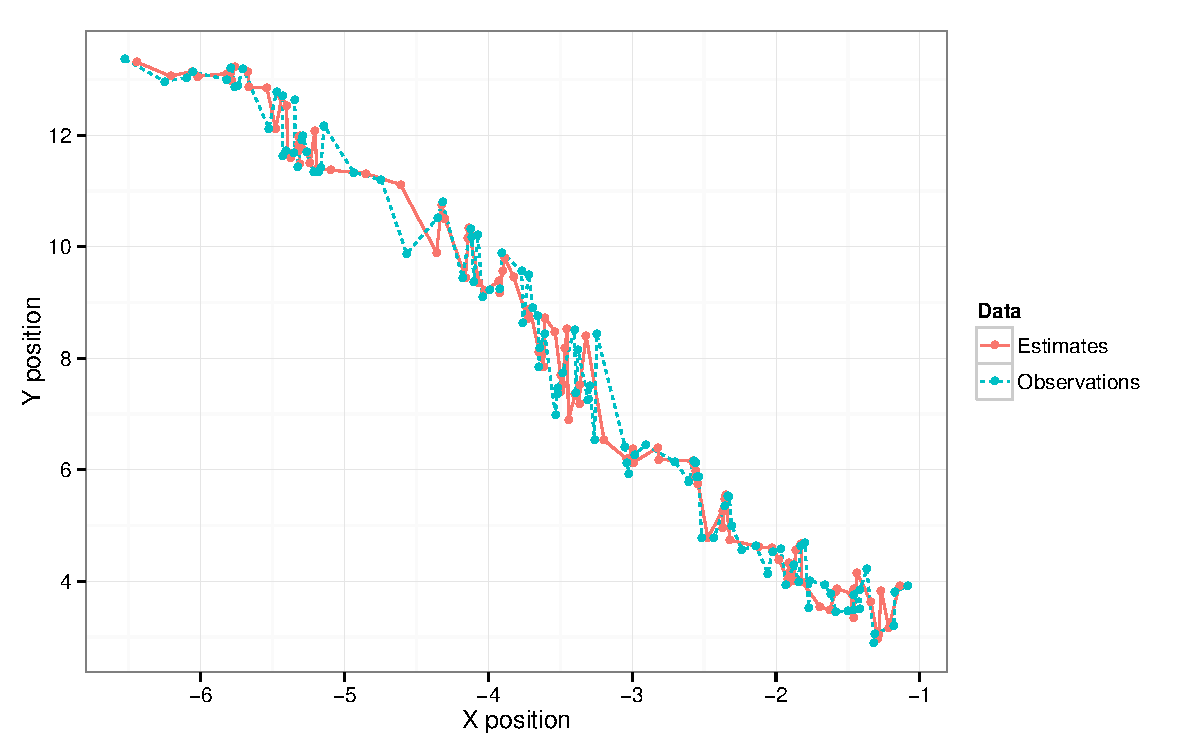
\includegraphics[width=\linewidth]{fig/pf}
  \caption{Observations and estimates of a simple particle filter.}
  \label{fig:pf}
\end{figure}

\subsection{Bayesian Modeling of Gaussian mixture model}
\label{sub:Bayesian Modeling of Gaussian mixture model}

\subsubsection{The model and algorithm}

Since \textcite{Richardson:1997ea}, the Gaussian mixture model (\gmm) has
provided a canonical example of a model-order-determination problem. We use
the same model as in \textcite{DelMoral:2006hc} to illustrate the
implementation of this classical example in Monte Carlo literature. This model
is also used in \textcite{Zhou2013mc} for demonstration of the use of \smc in
the context of Bayesian model comparison, which provides more details of the
following setting. The model is as the following, data $\bfy =
(y_1,\dots,y_n)$ are independently and identically distributed as
\begin{equation*}
  y_i|\theta_r \sim \sum_{j=1}^r \omega_j\calN(\mu_j,\lambda_j^{-1}),
\end{equation*}
where $\calN(\mu_j,\lambda_j^{-1})$ denotes the Normal distribution with mean
$\mu_j$ and precision $\lambda_j$; $\theta_r =
(\mu_{1:r},\lambda_{1:r},\omega_{1:r})$ and $r$ is the number of components in
each model. The parameter space is thus $\Real^r\times\Real^{+r}\times S_r$
where $S_r = \{\omega_{1:r}:0\le\omega_j\le1; \sum_{j=1}^r\omega_j=1\}$ is the
standard $(r-1)$-simplex. The priors which are the same for each component are
taken to be $\mu_j\sim\calN(\xi,\kappa^{-1})$, $\lambda_j\sim\calG(\nu,\chi)$
and $\omega_{1:r}\sim\calD(\rho)$ where $\calD(\rho)$ is the symmetric
Dirichlet distribution with parameter $\rho$ and $\calG(\nu,\chi)$ is the
Gamma distribution with shape $\nu$ and scale $\chi$. The prior parameters are
set in the same manner as in \textcite{Richardson:1997ea}; also see
\textcite{Zhou2013mc} for details. The data is simulated from a four
components model with $\mu_{1:4} = (-3, 0,3, 6)$, and $\lambda_j =2$,
$\omega_j = 0.25$, $j = 1,\dots,4$. Our interest is to simulate the posterior
distribution of models with $r$ components, denoted by $M_r$ and obtaining the
normalizing constant for the purpose of Bayesian model comparison
\textcite[chap.~7]{Robert:2007tc}.

Numerous strategies are possible to construct a sequence of distributions for
the purpose of \smc sampling. One option is to use for each model $M_r$,
$r\in\{1,2,\dots\}$, the sequence $\{\pi_t\}_{t=0}^{T_r}$, defined by
\begin{equation}
  \pi_t(\theta_r^t) \propto
  \pi(\theta_r^t|M_r)p(\bfy|\theta_r^t,M_r)^{\alpha(t/T_r)},
  \label{eq:geometry}
\end{equation}
where the number of distributions, $T_r$, and the annealing schedule,
$\alpha:[0,1]\to[0,1]$, may be different for each model. This leads to
algorithm~\ref{alg:gmm}.

\begin{algorithm}[t]
\begin{algorithmic}
  \hrule\vskip1ex
  \STATE For each model $M_r\in\calM$ perform the following algorithm.

  \STATE \emph{Initialization}
  \STATE\STATESKIP Set $t\leftarrow0$.
  \STATE\STATESKIP Sample $\theta_r^{(i,t)}\sim\pi(\theta_r^{(i,t)}|M_r)$.
  \STATE\STATESKIP Weight $W_0^{(i)} \propto 1$.

  \STATE \emph{Iteration}
  \STATE\STATESKIP Set $t\leftarrow t + 1$.
  \STATE\STATESKIP Weight $W_t^{(i)} \propto W_{t-1}^{(i)}
  p(\bfy|\theta_r^{(i,t-1)},M_r)^{\alpha(t/T_r) - \alpha([t-1]/T_r)}$.
  \STATE\STATESKIP Apply resampling if necessary.
  \STATE\STATESKIP Sample $\theta_r^{(i,t)} \sim
  K_t(\cdot|\theta_r^{(i,t-1)})$, a $\pi_t$-invariant \mcmc kernel.

  \STATE \emph{Repeat the \emph{Iteration} step up to $t = T_r$}.
  \vskip1ex\hrule
\end{algorithmic}
\caption{\smc algorithm for Bayesian modeling of Gaussian mixture
  model.}
\label{alg:gmm}
\end{algorithm}

The \mcmc kernel $K_t$ in algorithm~\ref{alg:gmm} is constructed as a
three-blocks Metropolis random walk,
\begin{enumerate}
  \item Update $\mu_{1:r}$ through a Normal random walk.
  \item Update $\lambda_{1:r}$ through a Normal random walk on logarithm
    scale, that is, on $\log\lambda_{j}$, $j = 1, \dots, r$.
  \item Update $\omega_{1:r}$ through a Normal random walk on logit scale,
    that is, on $\log(\omega_{j}/\omega_r)$, $j = 1,\dots,r-1$.
\end{enumerate}

The standard direct estimate of the normalizing constants
\textcite{DelMoral:2006hc} can be obtained from the output of this \smc
algorithm as,
\begin{equation}
  \hat\lambda_{\text{\textsc{ds}}}^{T_r,N} =
  \sum_{i=1}^N \frac{\pi(\theta_r^{(i,0)}|M_r)}{\nu(\theta_0^{(i,0)})} \times
  \prod_{t=1}^{T_r} \sum_{i=1}^N W_{t-1}^{(i)}
  p(\bfy|\theta_r^{(i,t)}M_r)^{\alpha(t/T_r) - \alpha([t-1]/T_r)},
  \label{eq:smc-ds}
\end{equation}
where $W_{t-1}^{(i)}$ is the importance weight of sample $\theta_{t-1}^{(i)}$.

\subsubsection{Path sampling for estimation of normalizing constants}

As shown in \textcite{Zhou2013mc} the estimation of the normalizing constant
associated with our sequence of distributions can also be achieved by a Monte
Carlo approximation to the \emph{path sampling} formulation given by
\textcite{Gelman:1998ei}, also known as thermodynamic integration or Ogata's
method. Given a parameter $\alpha$ which defines a family of distributions,
$\{p_{\alpha} = q_{\alpha} / Z_\alpha\}_{\alpha \in [0,1]}$ that moves
smoothly from $p_0 = q_0 / Z_0$ to $p_1 = q_1 / Z_1$ as $\alpha$ increases
from zero to one, one can estimate the logarithm of the ratio of their
normalizing constants via a simple integral relationship,
\begin{equation}
  \log\Round[bigg]{\frac{Z_1}{Z_0}} = \int_{0}^{1} \Exp_\alpha
  \Square[bigg]{\fracd{\log q_{\alpha}(\cdot)}{\alpha}} \intd\alpha,
  \label{eq:path_identity}
\end{equation}
where $\Exp_\alpha$ denotes expectation under $p_\alpha$. The sequence of
distributions in the \smc algorithm for this example can be interpreted as
belonging to such a family of distributions, with $\alpha = \alpha(t/T_r)$.

The \smc sampler provides us with a set of weighted samples obtained from a
sequence of distributions suitable for approximating this integral. At each
time $t$ we can obtain an estimate of the expectation within the integral via
the usual importance sampling estimator, and this integral can then be
approximated via a trapezoidal integration. In summary, the path sampling
estimator of the ratio of normalizing constants $\lambda^{T_r} =
\log(Z_1/Z_0)$ can be approximated by,
\begin{equation}
  \hat\lambda_{\text{\textsc{ps}}}^{T_r,N} = \sum_{t=1}^{T_r}
  \frac{1}{2}(\alpha_t - \alpha_{t - 1})(U_t^N + U_{t-1}^N),
  \label{eq:path_est}
\end{equation}
where
\begin{equation}
  U_t^N = \sum_{i=1}^N
  W_t^{(i)} \fracd{\log q_{\alpha}(X_t^{(i)})}{\alpha}
  \Bigm|_{\alpha = \alpha_t}.
  \label{eq:path_import}
\end{equation}

\subsubsection{Implementations}

In this example we will implement the following classes.
\begin{itemize}
  \item \cppinline{gmm_param} is a class that abstracts the parameters of the
    model, $\theta_r = (\mu_{1:r},\lambda_{1:r},\omega_{1:r})$.
  \item \cppinline{gmm_state} is the value collection class.
  \item \cppinline{gmm_init} is a class that implements operations used to
    initialize the sampler.
  \item \cppinline{gmm_move_smc} is a class that implements operations used to
    update the weights as well as selecting the random walk proposal scales
    and distribution parameter $\alpha(t/T_r)$.
  \item \cppinline{gmm_move_mu}, \cppinline{gmm_move_lambda} and
    \cppinline{gmm_move_weight} are classes that implement the random walks,
    each for one of the three blocks.
  \item \cppinline{gmm_path} is a class that implements monitors for the path
    sampling estimator. This class is similar to the importance sampling
    monitor introduced before. It is to be used with
    \cppinline{Sampler<gmm_state>::path_sampling}. Its interface requirement
    will be documented later.
  \item \cppinline{gmm_alpha_linear} and \cppinline{gmm_alpha_prior} are
    classes that implement two of the many possible annealing schemes,
    $\alpha(t/T_r) = t/T_r$ (linear) and $\alpha(t/T_r) = (t/T_r)^p$, $p > 1$
    (prior).
  \item And last, the \cppinline{main} function, which configures, initializes
    and iterates the sampler.
\end{itemize}

This example is considerably more complicated than the last one. Instead of
documenting all the implementation details, for many classes we will only show
the interfaces. In most cases, the implementations are straightforward as they
are either data member accessors or simple translation of mathematical
formulations. For member functions with more complex structures, detailed
explanation will be given. Interested readers can see the source
(\cppinline{vSMCExample/paper/src/paper_gmm.cpp}) for more details.

Later we will build both sequential and parallelized samplers. A few
configuration macros will be defined at compile time. For example, the
sequential sampler is compiled with the following header and macros,
\begin{cppcode}
#include <vsmc/smp/backend_seq.hpp>
#define BASE_SATE StateSEQ
#define BASE_INIT InitializeSEQ
#define BASE_MOVE MoveSEQ
#define BASE_PATH PathEvalSEQ
\end{cppcode}
The definitions of these macros will be changed at compile time to build
parallelized samplers. For example, when using \lopenmp parallelization, the
header \cppinline{backend_omp.hpp} will be used instead of
\cppinline{backend_seq.hpp}; and \cppinline{StateSEQ} will be changed to
\cppinline{StateOMP} along with similar changes to the other macros. In the
distributed source, this is configured by the \lcmake build system.

Again, we first introduce the \cppinline{main} function. The required headers
are the same as the last particle filter example in addition to the \smp
backend headers as described above. The following variables used in the
\cppinline{main} function will be set by user input.
\begin{cppcode}
int ParticleNum;
int AnnealingScheme;
int PriorPower;
int CompNum;
std::string DataFile;
\end{cppcode}
In the \cppinline{main} function, we will create objects that set the
distribution parameter $\alpha(t/T_r)$ at each iteration according to user
input of \cppinline{AnnealingScheme}. Below is the \cppinline{main} function.
Note that some code of \io operations which set the parameters above is
omitted.
\begin{cppcode}
int main ()
{
    gmm_move_smc::alpha_setter_type alpha_setter;
    if (AnnealingScheme == 1)
        alpha_setter = gmm_alpha_linear(IterNum);
    if (AnnealingScheme == 2)
        alpha_setter = gmm_alpha_prior(IterNum, PriorPower);

    Sampler<gmm_state> sampler(ParticleNum, Stratified, 0.5);
    sampler.particle().value().comp_num(CompNum);
    sampler
        .init(gmm_init());
        .move(gmm_move_smc(alpha_setter), false);
        .mcmc(gmm_move_mu(), false);
        .mcmc(gmm_move_lambda(), true);
        .mcmc(gmm_move_weight(), true);
        .path_sampling(gmm_path());
        .initialize((void *) DataFile.c_str());
        .iterate(IterNum);

    double ps = sampler.path().log_zconst();
    std::cout << "Path sampling estimate : " << ps << std::endl;

    return 0;
}
\end{cppcode}
The sampler first sets the number of components and allocates memory through
member function \cppinline{comp_num} of \cppinline{gmm_state}. Then it sets
the initialization and updating methods. Before possible resampling, a
\cppinline{gmm_move_smc} object is added. After that, three Metropolis random
walks are appended. In addition, we add a \cppinline{gmm_path} object to
calculate the path sampling integration. Then we initialize and iterate the
sampler and get the normalizing constant estimates.

It is obvious that the parameter class \cppinline{gmm_param} needs to store
the parameter vector $(\mu_{1:r},\lambda_{1:r},\omega_{1:r})$. We also
associate with each particle its log-likelihood and log-prior. Here is the
definition of the \cppinline{gmm_param} class. We omitted definitions of some
data access member functions.
\begin{cppcode}
class gmm_param
{
    public :

    void comp_num (std::size_t num);
    void save_old ();

    double log_prior () const {return log_prior_;}
    double &log_prior () {return log_prior_;}

    double log_likelihood () const {return log_likelihood_;}
    double &log_likelihood () {return log_likelihood_;}

    int mh_reject_mu (double p, double u);
    int mh_reject_lambda (double p, double u);
    int mh_reject_weight (double p, double u);
    int mh_reject_common (double p, double u);

    double log_lambda_diff () const;
    double logit_weight_diff () const;

    void update_log_lambda ();

    private :

    std::size_t comp_num_;
    double log_prior_, log_prior_old_, log_likelihood_, log_likelihood_old_;
    std::vector<double> mu_, mu_old_;
    std::vector<double> lambda_, lambda_old_;
    std::vector<double> weight_, weight_old_;
    std::vector<double> log_lambda_;
};
\end{cppcode}
The \cppinline{comp_num} member function allocates the memory for a given
number of components. The \cppinline{save_old} member function save the
current particle states. It is used before the states are updated with the
random walk proposals, as we will see later when we implement the
\cppinline{gmm_move_mu} class. The \cppinline{mh_reject_mu} member function
accepts the Metropolis acceptance probability $p$ and a uniform $(0,1]$ random
variate, say $u$; it rejects the proposed change if $p < u$, and restore the
particle state of the parameters $\mu_{1:r}$ with those saved by
\cppinline{save_old}. The member functions \cppinline{mh_reject_lambda} and
\cppinline{mh_reject_weight} do the same for the other two sets of parameters.
All these three also call the \cppinline{mh_reject_common} which restore the
stored log-likelihood and log-prior values. The use of these member functions
will be seen in the implementation of \cppinline{gmm_move_mu}, in the context
of which their own implementation become obvious. Other member functions
provide some useful computations such as the logarithm of the $\lambda_{1:r}$.
They are used when compute the log-likelihood.

The class \cppinline{gmm_state} contains some properties common to all
particles, such as the data and the distribution parameter $\alpha(t/T_r)$.
The prior parameters are also stored in the value collection. Here is the
definition of this value collection class. Again, we omitted some data access
member functions,
\begin{cppcode}
class gmm_state : public BASE_STATE<StateMatrix<RowMajor, 1, gmm_param> >
{
    public :

    void alpha (double a)
    {
        a = a < 1 ? a : 1;
        a = a > 0 ? a : 0;
        if (a == 0) {
            alpha_inc_ = 0;
            alpha_ = 0;
        } else {
            alpha_inc_ = a - alpha_;
            alpha_ = a;
        }
    }

    void comp_num (std::size_t num)
    {
        comp_num_ = num;
        for (size_type i = 0; i != this->size(); ++i)
            this->state(i, 0).comp_num(num);
    }

    double update_log_prior (gmm_param &param) const;

    double update_log_likelihood (gmm_param &param) const
    {
        const double log2pi = 1.8378770664093455;
        double ll = -0.5 * obs_.size() * log2pi;
        param.update_log_lambda();
        for (std::size_t k = 0; k != obs_.size(); ++k) {
            double lli = 0;
            for (std::size_t i = 0; i != param.comp_num(); ++i) {
                double resid = obs_[k] - param.mu(i);
                lli += param.weight(i) * std::exp(
                        0.5 * param.log_lambda(i) -
                        0.5 * param.lambda(i) * resid * resid);
            }
            ll += std::log(lli);
        }

        return param.log_likelihood() = ll;
    }

    void read_data (const char *filename);

    private :

    std::size_t comp_num_;
    double alpha_, alpha_inc_;
    double mu0_, sd0_, shape0_, scale0_;
    double mu_sd_, lambda_sd_, weight_sd_;
    std::vector<double> obs_;
};
\end{cppcode}
The variable \cppinline{alpha_inc_} is $\Delta\alpha(t/T_r) = \alpha(t/T_r) -
\alpha((t-1)/T_r)$, which will be used when we update the weights. The
variables \cppinline{mu0_} and \cppinline{sd0_} are the prior parameters of
the means $\mu_{1:r}$. The variables \cppinline{shape0_} and
\cppinline{scale0_} are the prior parameters of the precisions
$\lambda_{1:r}$. The variables \cppinline{mu_sd_}, \cppinline{lambda_sd_}, and
\cppinline{weight_sd_} are the proposal scales of the three random walks,
respectively. The data access member functions of these variables are omitted
in the above code snippet.

In the \cppinline{update_log_likelihood} member function, the calculation is a
straightforward translation of the mathematical formulation. The
\cppinline{gmm_param::update_log_lambda} member function is used before the
loop, which simply calculates $\log\lambda_j$ for $j = 1,\dots,r$, and stores
their values. The purpose is to avoid repeated computation of these quantities
inside the loop. When the function returns, it uses the mutable version of the
\cppinline{gmm_param::log_likelihood} member function to update the
log-likelihood stored in the \cppinline{param} object. This is the reason that
the function is named with an \cppinline{update} prefix. As we will see later,
whenever the parameter values are updated, it will be followed by a call to
\cppinline{update_log_likelihood} and \cppinline{update_log_prior}, which is
implemented in a similar fashion. Therefore the value we get by calling
\cppinline{gmm_param::log_likelihood} will always be ``up-to-date'' while no
repeated computation is involved. Surely there are other and possibly better
design choices. However, for this simple example, this design serves our
purpose well.

The initialization is implemented using the \cppinline{gmm_init} class,
\begin{cppcode}
class gmm_init : public BASE_INIT<gmm_state, gmm_init>
{
    public :

    std::size_t initialize_state (SingleParticle<gmm_state> sp)
    {
        const gmm_state &state = sp.particle().value();
        gmm_param &param = sp.state(0);

        cxx11::normal_distribution<> rmu(
                state.mu0(), state.sd0());
        cxx11::gamma_distribution<> rlambda(
                state.shape0(), state.scale0());
        cxx11::gamma_distribution<> rweight(1, 1);

        double sum = 0;
        for (std::size_t i = 0; i != param.comp_num(); ++i) {
            param.mu(i)     = rmu(sp.rng());
            param.lambda(i) = rlambda(sp.rng());
            param.weight(i) = rweight(sp.rng());
            sum += param.weight(i);
        }
        for (std::size_t i = 0; i != param.comp_num(); ++i)
            param.weight(i) /= sum;

        state.update_log_prior(param);
        state.update_log_likelihood(param);

        return 1;
    }

    void initialize_param (Particle<gmm_state> &particle,
                           void *filename)
    {
        if (filename)
            particle.value().read_data(static_cast<const char *>(filename));
        particle.value().alpha(0);
        particle.set_equal_weight();
    }
};
\end{cppcode}
The \cppinline{initialize_param} member function is called before the
\cppinline{pre_processor}, which is absent in this case and have the default
implementation which does nothing. It processes the optional parameter of
\cppinline{Sampler::initialize}, the file name of the data. The
\cppinline{initialize_state} member function initialize the state values
according to the prior and update the log-prior and log-likelihood.

After initialization, at each iteration, \cppinline{gmm_move_smc} class will
implement the updating of weights as well as the selecting of the proposal
scales and the distribution parameter. For example, when using the linear
annealing scheme, we can implement a \cppinline{gmm_alpha_linear} class as the
following,
\begin{cppcode}
class gmm_alpha_linear
{
    public :

    gmm_alpha_linear (const std::size_t iter_num) : iter_num_(iter_num) {}

    void operator() (std::size_t iter, Particle<gmm_state> &particle)
    {particle.value().alpha(static_cast<double>(iter) / iter_num_);}

    private :

    std::size_t iter_num_;
};
\end{cppcode}
It accepts the total number of iterations $T_r$ as an argument to its
constructor. And it implements an \cppinline{operator()} that updates the
distribution parameter $\alpha(t/T_r)$. The prior annealing scheme can be
implemented similarly. For simplicity and demonstration purpose, we only allow
\cppinline{gmm_move_smc} to be configured with different annealing schemes,
and hard code the proposal scales. An industry strength design may make this
class a template with annealing scheme and proposal scales as policy template
parameters.
\begin{cppcode}
class gmm_move_smc
{
    public :

    typedef cxx11::function<void (std::size_t, Particle<gmm_state> &)>
        alpha_setter_type;

    gmm_move_smc (const alpha_setter_type &alpha_setter) :
        alpha_setter_(alpha_setter) {}

    std::size_t operator() (std::size_t iter, Particle<gmm_state> &particle)
    {
        alpha_setter_(iter, particle);

        double alpha = particle.value().alpha();
        alpha = alpha < 0.02 ? 0.02 : alpha;
        particle.value().mu_sd(0.15 / alpha);
        particle.value().lambda_sd((1 + std::sqrt(1 / alpha)) * 0.15);
        particle.value().weight_sd((1 + std::sqrt(1 / alpha)) * 0.2);

        incw_.resize(particle.size());
        weight_.resize(particle.size());
        particle.read_weight(weight_.begin());
        double coeff = particle.value().alpha_inc();
        for (Particle<gmm_state>::size_type i = 0;
                i != particle.size(); ++i) {
            incw_[i] =
                coeff * particle.value().state(i, 0).log_likelihood();
        }
        particle.weight_set().add_log_weight(&incw_[0]);

        return 0;
    }

    private :

    alpha_setter_type alpha_setter_;
    std::vector<double> incw_;
    std::vector<double> weight_;
};
\end{cppcode}
Note that, \cppinline{cxx11::function} is an alias to either
\cppinline{std::function} or \cppinline{boost::function}, depending on the
value of the configuration macro \cppinline{VSMC_HAS_CXX11LIB_FUNCTIONAL}.
Objects of this class type can be added to a sampler as a move. The
\cppinline{operator()} satisfies the interface requirement of the core module.
First it uses \cppinline{alpha_setter_} to set the distribution parameter
$\alpha(t/T_r)$. Second, it sets the proposal scales for the three Metropolis
random walks according to the current value of $\alpha$. Then it computes the
\emph{unnormalized} incremental weights. The last, we also modify the
\cppinline{WeightSet} type object itself by adding the logarithm of the
incremental weights.

At each iteration, random walks are also performed. The implementations of the
random walks are straightforward. Below is the implementation of the random
walk on the mean parameters. The random walks on the other parameters are
similar.
\begin{cppcode}
class gmm_move_mu : public BASE_MOVE<gmm_state, gmm_move_mu>
{
    public :

    std::size_t move_state (std::size_t iter, SingleParticle<gmm_state> sp)
    {
        const gmm_state &state = sp.particle().value();
        gmm_param &param = sp.state(0);

        cxx11::normal_distribution<> rmu(0, state.mu_sd());
        cxx11::uniform_real_distribution<> runif(0, 1);

        double p =
            param.log_prior() + state.alpha() * param.log_likelihood();
        param.save_old();
        for (std::size_t i = 0; i != param.comp_num(); ++i)
            param.mu(i) += rmu(sp.rng());
        p = state.update_log_prior(param) +
            state.alpha() * state.update_log_likelihood(param) - p;
        double u = std::log(runif(sp.rng()));

        return param.mh_reject_mu(p, u);
    }
};
\end{cppcode}
First we save the logarithm of the value of target density computed using the
old values in \cppinline{p}, the acceptance probability. And then we call
\cppinline{gmm_param::save_old} to save the old values. Next we update each
parameter with a proposed Normal random variates and compute the new log-prior
and the log-likelihood as well as the new value of the target density. Then we
reject it according to the Metropolis algorithm, as implemented in
\cppinline{gmm_param}, which manages both the current states as well as the
backup.

Last we need to monitor certain quantities for inference purpose. Recall that,
in the \cppinline{main} function we used
\cppinline{sampler.path_sampling(gmm_path())} to set the monitoring of path
sampling integrands. The \cppinline{path_sampling} member function requires a
callable objects with the following signature,
\begin{cppcode}
double path_eval (std::size_t iter, const Particle<T> &, double *res);
\end{cppcode}
The input parameter \cppinline{iter} is the iteration number, the value of $t$
in Equation~\ref{eq:path_est}. The return value shall be the value of
$\alpha_t$. The output parameter \cppinline{res} shall store the array of
values
\begin{equation*}
  \fracd{\log q_{\alpha}(X_t^{(i)})}{\alpha}\Bigm|_{\alpha = \alpha_t}.
\end{equation*}
Our implementation of \cppinline{gmm_path} is a subclass of an \smp module
base class, which provides an \cppinline{operator()} that satisfies the above
interface requirement. Its usage is similar to the \cppinline{MoveSEQ}
template introduced in section~\ref{sub:SMP module}.

The path sampling integrands under this geometry annealing scheme are simply
the log-likelihood. Therefore the implementation of \cppinline{gmm_path} class
is rather simple,
\begin{cppcode}
class gmm_path : public BASE_PATH<gmm_state, gmm_path>
{
    public :

    double path_state (std::size_t, ConstSingleParticle<gmm_state> sp)
    {return sp.state(0).log_likelihood();}

    double path_grid (std::size_t, const Particle<gmm_state> &particle)
    {return particle.value().alpha();}
};
\end{cppcode}

\subsubsection{Results}

After compiling and running the algorithm, the results were consistent with
those reported in \textcite{DelMoral:2006hc}. For a more in depth analyze of
the methodologies, extensions and the results see \textcite{Zhou2013mc}.

\subsubsection{Extending the implementation using \protect\mpi}

\vsmc's \lmpi module assumes that identical samplers are constructed on each
node, with possible different number of particles to accommodate the
difference in capacities among nodes. To extend the above \smp implementation
for use with \lmpi, first at the beginning of the \cppinline{main} function,
we add the following,
\begin{cppcode}
MPIEnvironment env(argc, argv);
\end{cppcode}
to initialize the \lmpi environment. When the object \cppinline{env} is
destroyed at the exit of the \cppinline{main} function, the \lmpi environment
is finalized. Second, we need to replace base value collection class template
with \cppinline{StateMPI}. So now \cppinline{gmm_state} is declared as the
following,
\begin{cppcode}
class gmm_state :
    public StateMPI<BASE_STATE<StateMatrix<RowMajor, 1, gmm_param> > >;
\end{cppcode}
The implementation is exactly the same as before. Third, the
\cppinline{gmm_param} class now needs to be transferable using \lmpi. Unlike
the \smp situations, a simple copy constructor is not enough. \vsmc uses
\lboost \lmpi library, and thus one only needs to write a
\cppinline{serialize} member function for \cppinline{gmm_param} such that the
data can be serialized into bytes. See documents of \lboost \lmpi and
serialization libraries for details. In summary, the following member function
accepts an \cppinline{Archive} object as input, and it can perform a store or
a load operation based on the \cppinline{Archive} type. In a load operation,
the \cppinline{Archive} object is like an input stream and in a store
operation, it is like an output stream.
\begin{cppcode}
template <typename Archive>
void serialize (Archive &ar, const unsigned)
{
    int num = comp_num_;
    ar & num;
    comp_num(num);

    ar & log_prior_;
    ar & log_likelihood_;
    for (std::size_t i = 0; i != comp_num_; ++i) {
        ar & mu_[i];
        ar & lambda_[i];
        ar & weight_[i];
        ar & log_lambda_[i];
    }
}
\end{cppcode}
Fourth, after user input of the sampler parameters, we need to sync them with
all nodes. For example, for the \cppinline{ParticleNum} parameter,
\begin{cppcode}
boost::mpi::communicator World;
boost::mpi::broadcast(World, ParticleNum, 0);
\end{cppcode}
Last, any importance sampling estimates that are computed on each node, need
to be combined into final results. For example, the path sampling results are
now obtained through adding the results from each node together,
\begin{cppcode}
double ps_sum = 0;
boost::mpi::reduce(World, ps, ps_sum, std::plus<double>(), 0);
ps = ps_sum;
\end{cppcode}

After these few lines of change, the sampler is now parallelized using \lmpi
and can be deployed to clusters and other distributed memory architecture. On
each node, the selected \smp parallelization is used to perform
multi-threading parallelization locally. \vsmc's \lmpi module will take care
of normalizing weights and other tasks.

\subsubsection{Parallelization performance}

One of the main motivation behind the creation of \vsmc is to ease the
parallelization with different programming models. The same implementation can
be used to built different samplers based on what kind of parallel programming
model is supported on users' platforms. In this section we compare the
performance of various \smp parallel programming models and \lopencl
parallelization.

We consider five different implementations supported by \licpc 2013:
sequential, \ltbb, \lcilk, \lopenmp and \cppoo \cppinline{<thread>}. The
samplers are compiled with
\begin{cppcode}
CXX=icpc -std=c++11 -gcc-name=gcc-4.7 -gxx-name=g++-4.7
CXXFLAGS=-O3 -xHost -fp-model precise  \
         -DVSMC_HAS_CXX11LIB_FUNCTIONAL=1  \
         -DVSMC_HAS_CXX11LIB_RANDOM=1
\end{cppcode}
on a Ubuntu~12.10 workstation with an Xeon W3550 (3.06GHz, 4 cores, 8 hardware
threads through hyper-threading) \cpu. A four components model and $100$
iterations with a prior annealing scheme is used for all implementations. A
range of numbers of particles are tested, from $2^3$ to $2^{17}$.

For different number of particles, the wall clock time and speedup are shown
in figure~\ref{fig:bench-smp-perf}. For $10^4$ or more particles, the
differences are minimal among all the programming models. They all have
roughly 550\% speedup. With smaller number of particles, \vsmc's \cppoo
parallelization is less efficient than other industry strength programming
models. However, with $1000$ or more particles, which is less than those used
typical applications, the difference is not very significant.

\begin{figure}
  \centering
  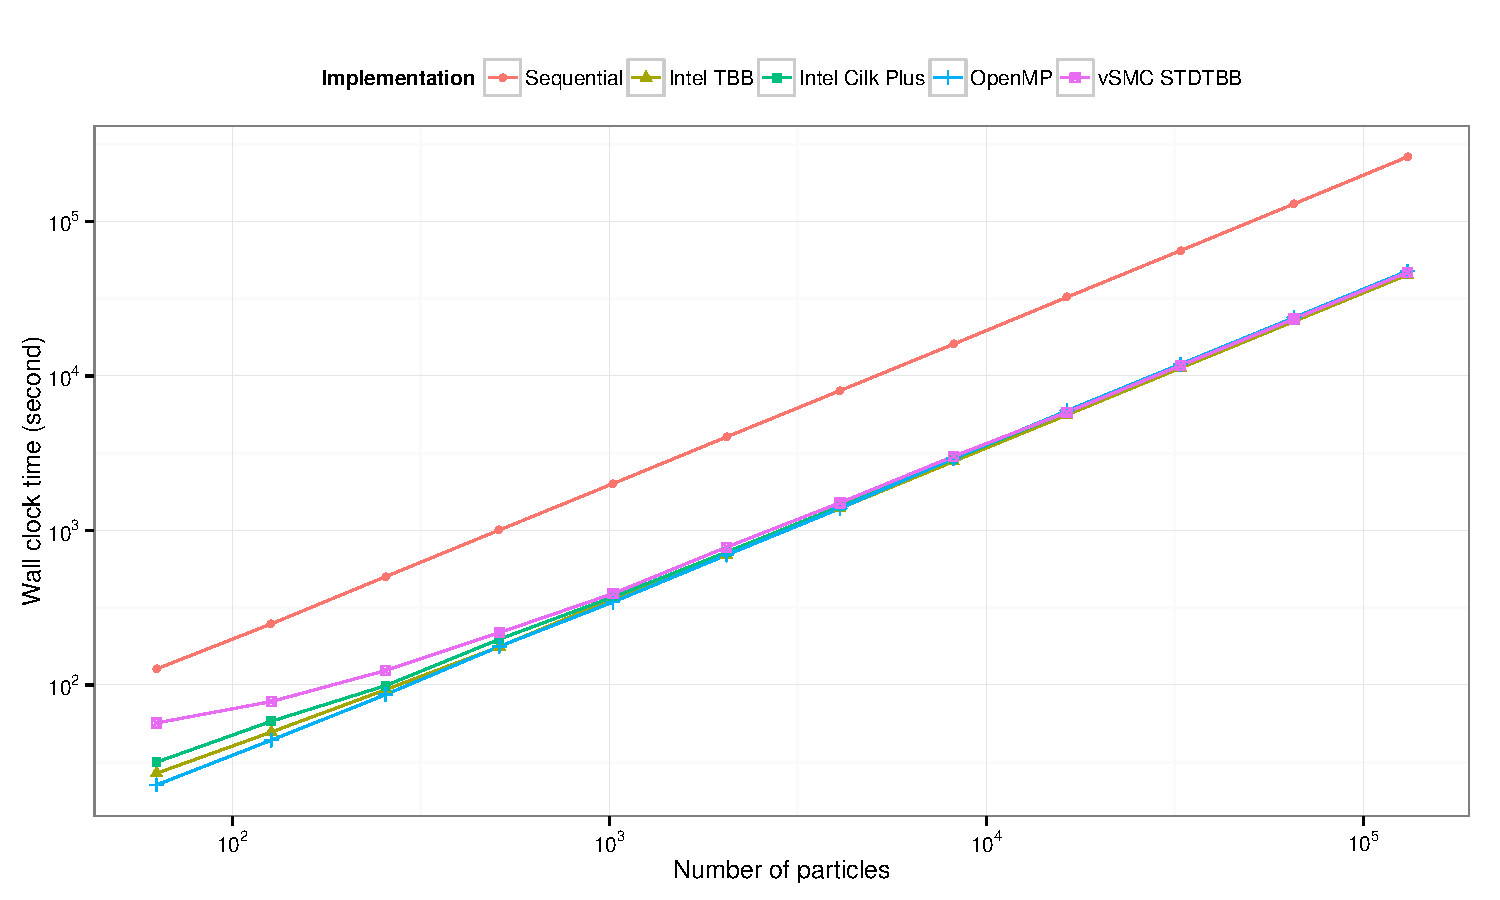
\includegraphics[width=\linewidth]{fig/bench-smp-time-running}
  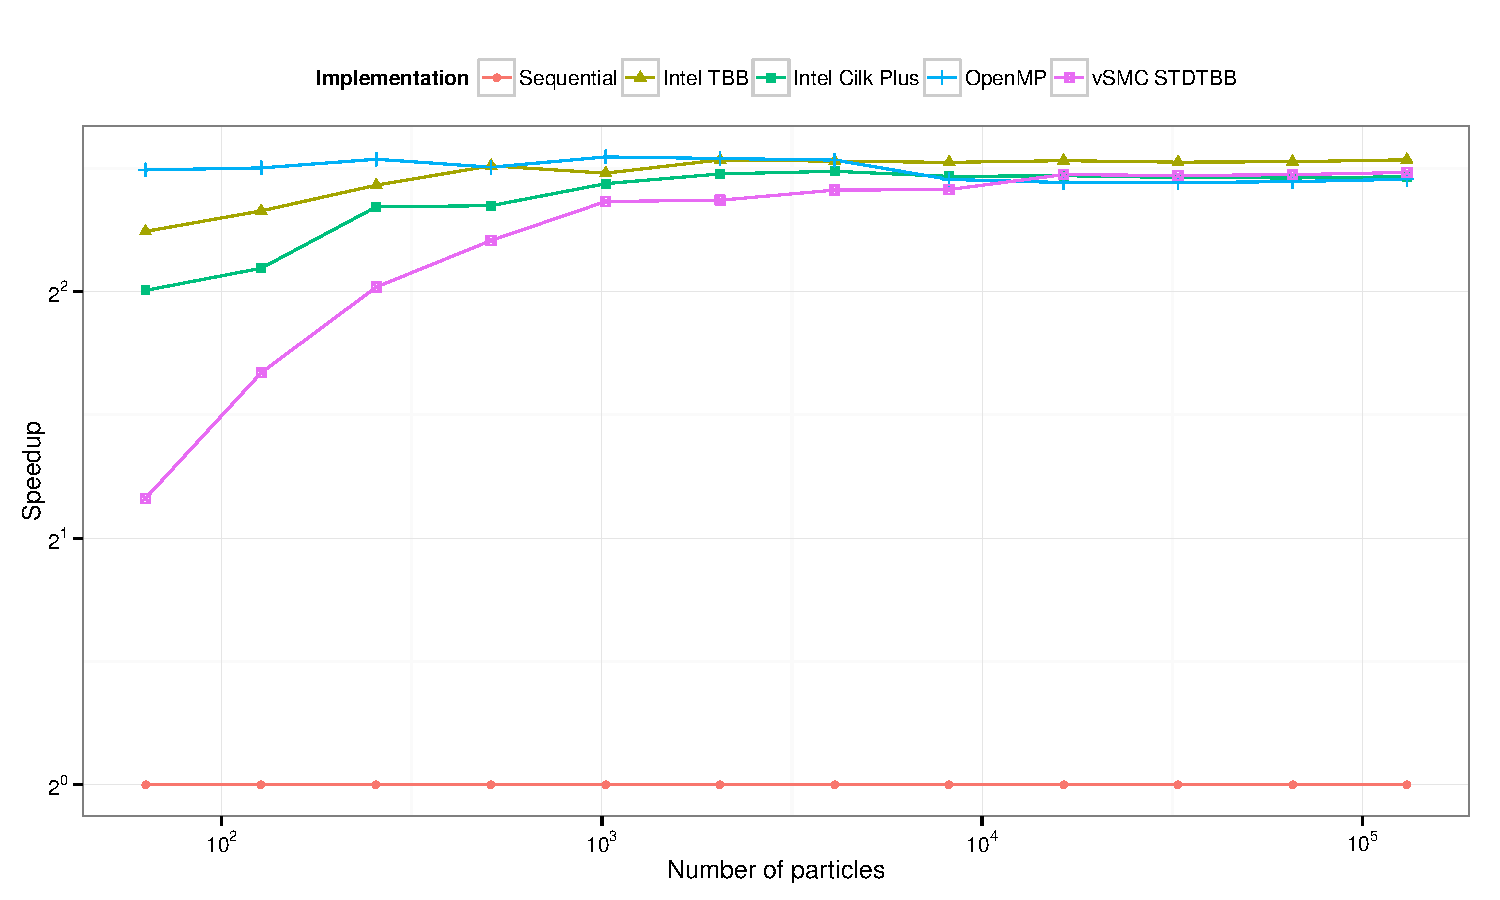
\includegraphics[width=\linewidth]{fig/bench-smp-speedup-running}
  \caption{Performance of \cpp implementations of Bayesian modeling for
    Gaussian mixture model (Linux; Xeon W3550, 3.06GHz, 4 cores, 8 threads).}
  \label{fig:bench-smp-perf}
\end{figure}

\begin{figure}
  \centering
  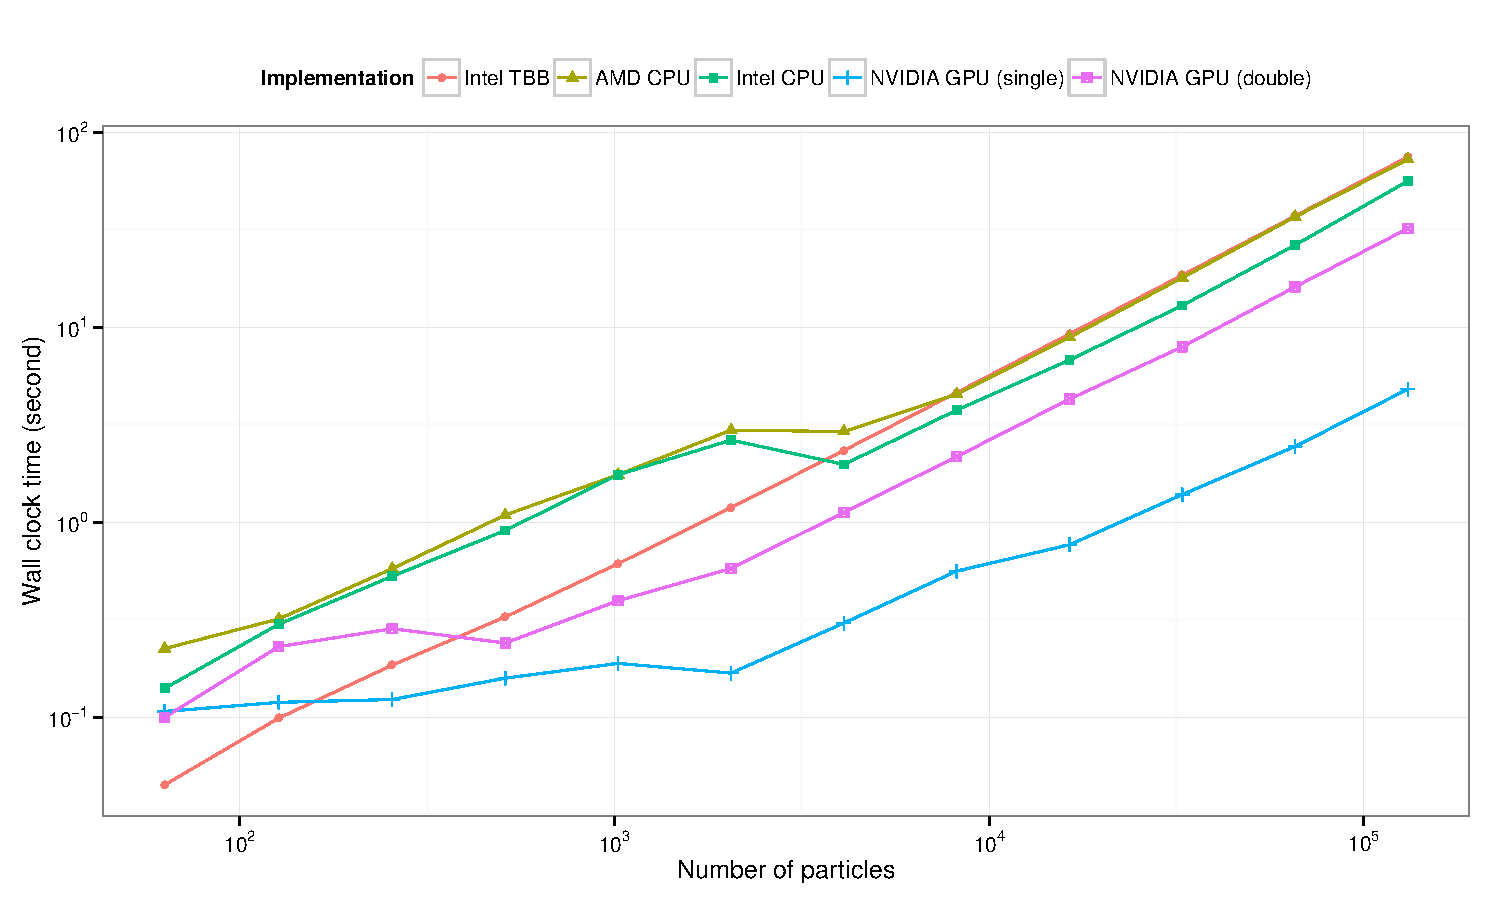
\includegraphics[width=\linewidth]{fig/bench-ocl-time-running}
  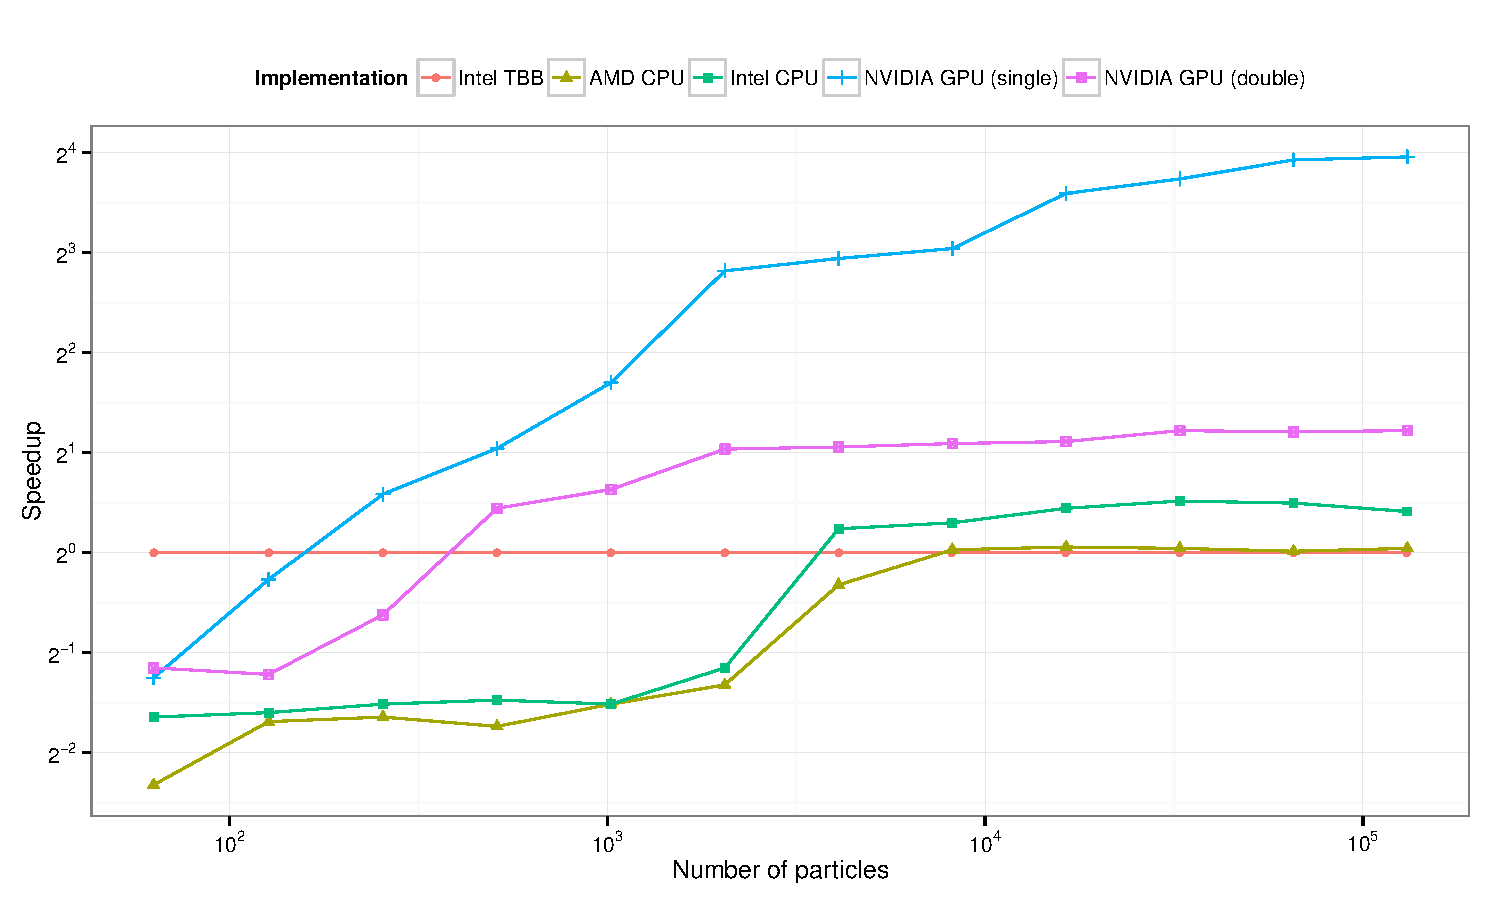
\includegraphics[width=\linewidth]{fig/bench-ocl-speedup-running}
  \caption{Performance of \lopencl implementations of Bayesian modeling for
    Gaussian mixture model (Linux; Xeon W3550 \gpu, 3.06GHz, 4 cores, 8
    threads; NVIDIA Quadro 2000).}
  \label{fig:bench-ocl-perf}
\end{figure}

\lopencl implementations are also compared on the same workstation, which also
has an NVIDIA Quadro 2000 graphic card. \lopencl programs can be compiled to
run on both \cpu{}s and \gpu{}s. For \cpu implementation, there are \fiocl and
\faocl platforms. We use the \ltbb implementation as a baseline for
comparison.  The same \lopencl implementation are used for all the \cpu and
\gpu runtimes.  Therefore they are not particularly optimized for any of them.
For the \gpu implementation, in addition to double precision, we also tested a
single precision configuration. Unlike modern \cpu{}s, which have the same
performance for double and single precision floating point operations (unless
\simd), \gpu{}s penalize double precision performance heavily.

For different number of particles, the wall clock time and speed up are
plotted in figure~\ref{fig:bench-ocl-perf}. With smaller number of particles,
the \lopencl implementations have a high overhead when compared to the \ltbb
implementation. With a large number of particles, \laocl has a similar
performance as the \ltbb implementation. \liocl is about 40\% faster than the
\ltbb implementation. This is due to more efficient vectorization and compiler
optimizations. The double precision performance of the NVIDIA \gpu has a 220\%
speedup and the single precision performance has near 1600\% speedup. As a
rough reference for the expected performance gain, the \cpu has a theoretical
peak performance of 24.48 GFLOPS. The \gpu has a theoretical peak performance
of 60 GFLOPS in double precision and 480 GFLOPS in single precision. This
represents 245\% and 1960\% speedup compared to the \cpu, respectively.

It is widely believed that \lopencl programming is tedious and hard. However,
\vsmc provides facilities to manage \lopencl platforms and devices as well as
common operations. Limited by the scope of this paper, the \lopencl
implementation (distributed with the \vsmc source) is not documented in this
paper. Overall the \lopencl implementation has about 800 lines including both
host and device code. It is not an enormous increase in effort when compared
to the 500 lines \smp implementation. Less than doubling the code base but
gaining more than 15 times performance speedup, we consider the programming
effort is relatively small.

\section{Discussion}
\label{sec:Discussion}

This paper introduced a \cpp template library intended for implementing
generic \smc algorithms and constructing parallel samplers with different
programming models. While it is possible to implement many realistic
applications with the presented framework, some technical proficiency is still
required to implement some problem specific part of the algorithms. Some basic
knowledge of \cpp in general and how to use a template library are also
required.

It is shown that with the presented framework it is possible to implement
parallelized, scalable \smc samplers in an efficient and reusable way. The
performance of some common parallel programming models are compared using an
example.

Some future work may worth the effort to ease the implementation of \smc
algorithms further. However, there is a balance between performance,
flexibility and the ease of use. \vsmc aims to be developer-friendly and to
provide users as much control as possible for all performance related aspects.
For a \lbugs-like interface, users may be interested in other software such as
\fbiips \parencite{BiiPS}. In addition \flibbi \parencite{Murray2013bi}
provides a user friendly and high performance alternative with a focus on
state-space models. Compared with these recent developments, \vsmc is less
accessible to those with little or no knowledge of \cpp. However, for
researchers with expertise in \cpp and template metaprogramming in particular,
\vsmc provides a framework within which potential superior performance can be
obtained and greater flexibility and extensibility are possible.

\clearpage
\appendix

\section[vSMC and SMCTC]{\protect\vsmc and \protect\smctc}
\label{sec:vsmc and smctc}

As noted by one referee, it is of interest to compare the \vsmc and \lsmctc
libraries. In particular, the differences and advantages of \vsmc when
parallel computing is not involved.

As mentioned in section~\ref{sec:Introduction}, the \vsmc library has some
similarity to \lsmctc. This is by intention so users already familiar with
\lsmctc can learn the new library easier. For example, they both use user
defined type to abstract algorithm specific state space. They also both use
user defined callbacks to perform algorithm specific operations such as
updating particles. However there are also differences.

The most significant difference is perhaps how the particle system is
abstracted. In \lsmctc, users write custom classes to abstract $X^{(i)}$. In
\vsmc, users define classes to abstract $\{X^{(i)}\}_{i=1}^N$. In addition, in
\lsmctc user defined callbacks operate on each particle individually while in
\vsmc they operate on all particles as a whole. This design of \vsmc allows
different parallelization models to be implemented. For example, suppose that
\simd vectorization is desired, which is not currently directly supported by
\vsmc, one only need to implement the value collection type such that the
values are properly aligned in memory and in each callback, \simd operations
can be applied to the whole value collection since the \vsmc interface allows
users to access them all at once. This kind of constructs is not possible in
\lsmctc without changing the internal of the library. See also
section~\ref{sub:Core module} on the value collection type of \vsmc.

Apart from parallelization, \vsmc also has other advantages. Internally it has
a very different design to that of \lsmctc. It is more modular and almost all
parts of the sampler can be replaced without changing the internal of the
library. For example, consider that a new resampling algorithm is desired. In
\lsmctc, if it is not provided by the library, users have to implement all the
operations ranging from generating replication numbers to copying each
particle. In \vsmc, one only needs to implement a function with the following
signature,
\begin{cppcode}
template <typename SizeType>
void resample (std::size_t N, const double *weight, SizeType *copy_from);
\end{cppcode}
which given the normalized weights generates the number of replicates of each
particle. And in the \cppinline{Sampler}'s constructor, one pass it this
object instead of the name of the built-in resampling scheme name. \vsmc's
implementations of gathering the normalized weights into an array, and copying
particles according to the replication numbers can be reused. This particular
example is of interest when the sampler is parallelized using \lmpi, where
copying particles across all nodes requires some effort that may not be
trivial. On the other hand, if an existing resampling algorithm is sufficient,
but the parallelization requires special memory management, all one needs to
do is providing \vsmc with a specialized \cppinline{copy} member function
inside their value collection class. And the implementation of the resampling
can be reused. (This is exactly what \vsmc does for the \lopencl and \lmpi
module.)

In some situations, \lsmctc might appear to be easier to use than \vsmc. For
example, it allows one to define a class that abstracts a single particle. And
naturally such classes can easily define operations that manipulate a single
particle. In contrast, in \vsmc users can only interact with a single particle
through the \cppinline{SingleParticle<T>} object. However, as shown in
section~\ref{sub:SMP module}, users can obtain similar effects by defining the
\cppinline{single_particle_type} class template inside the value collection
type. Alternatively, one can also reuse classes defined for \lsmctc by
combining them with \cppinline{StateMatrix} or \cppinline{StateTuple}. The
\cppinline{single_particle_type} and resampling example are only two of many
places where \vsmc allows users to extend or replace its default
implementations. Through the use of template metaprogramming, \vsmc is much
more flexible than \lsmctc.

In summary, \vsmc aims to be as flexible as possible. To quote Larry Wall,
``Easy things should be easy, and hard things should be possible''. In \vsmc,
this means when some standard algorithm design is used, for example a common
resampling algorithm such as stratified resampling, it should be as easy as
passing a parameter to a \vsmc function. When the algorithm is not directly
supported by the library, users can replace \vsmc's implementation without
knowing the internal of the library while reusing as much as possible the rest
of the library. For example, the library can be used to implement population
\mcmc algorithms, such as those used in \textcite{Calderhead:2009bd} for
Bayesian model comparison. In addition, when multiple algorithms share common
operations, such as \mcmc kernels, they can be implemented once and shared
between different algorithms easily. See the examples distributed with the
source, where an \smc and a population \mcmc implementation of the same \gmm
model share a large amount of code.

\vsmc also enjoys higher performance even for sequential implementations. For
instance, as noted before, a sequential implementation in \vsmc of the
particle filter in section~\ref{sub:A simple particle filter} is about twice
faster than that in \lsmctc.

In the author's opinion, \lsmctc is suitable for implementing algorithms that
can fit into its framework easily. In contrast, \vsmc might be more suitable
for developing new algorithms, especially those related to \smc. \vsmc is also
useful when different parallelization of the same algorithm is desired. For
example, it is not uncommon that a new algorithm is developed on a personal
computer, which only has access to multicore parallelization, and tested using
small sample or data size. And later the same algorithm is deployed to a
distributed system for solving large problems. Using \vsmc, much of the
implementation can be reused during the production phase. It is also clear
that \vsmc has the potential to provide better performance. The last but not
least, though no software can be said to be ``future-proof'', it is possible
to enhance \vsmc with new parallel programming models while reusing existing
implementations of algorithms.

\printbibliography[heading=reference]

\end{document}
